\documentclass[twoside]{article}
\usepackage{icml2016}

% If your paper is accepted, change the options for the package
% aistats2015 as follows:
%
%\usepackage[accepted]{aistats2015}
%
% This option will print headings for the title of your paper and
% headings for the authors names, plus a copyright note at the end of
% the first column of the first page.

%%%%%%%%%%%%%%%%%%%%%%%%%%%%%%%%%%%%%%%%%%%%%%%%%%%%%%%%%%%%%%%%%%%%%%%%%%%%%%%%

\usepackage{amsmath}
\usepackage{amssymb}
\usepackage{amsthm}
\usepackage{mathtools}
\usepackage{graphicx}
\usepackage{rotating}
\usepackage{xcolor}
\usepackage[inline]{enumitem}

%\usepackage{algorithm}
%\usepackage[noend]{algpseudocode}
%\usepackage{algorithmicx}
%\usepackage{algorithm2e}

%\usepackage[authordate,bibencoding=auto,strict,backend=biber,natbib]{biblatex-chicago}
%\usepackage[round]{natbib}   % omit 'round' option if you prefer square brackets
%\bibliographystyle{plainnat}

\usepackage{tikz}
\usepackage{pgfplots}
\pgfplotsset{width=7cm,compat=1.8}
\definecolor{darkgreen}{RGB}{0,127,0}

%%%%%%%%%%%%%%%%%%%%%%%%%%%%%%%%%%%%%%%%

\newtheorem{cor}{Corallary}
\newtheorem{theorem}{Theorem}
\newtheorem{lemma}{Lemma}
\newtheorem{assumption}{Condition}
\newtheorem{defn}{Definition}

\DeclareMathOperator*{\argmin}{arg\,min}
\DeclareMathOperator*{\argmax}{arg\,max}
\DeclareMathOperator*{\vecspan}{span}
\DeclareMathOperator*{\affspan}{aff}
\DeclareMathOperator*{\subG}{subG}
\DeclareMathOperator*{\tr}{tr}

%\newcommand{\smin}[1]{s_\text{min}({#1})}
\newcommand{\smin}{s_\text{min}}
\newcommand{\smax}{s_\text{max}}
\newcommand{\qhi}{q_\text{hi}}
\newcommand{\qlo}{q_\text{lo}}
\newcommand{\zero}{\text{\textbf{0}}}
\newcommand{\Zproj}{Z^{\textit{proj}}}
\newcommand{\Zowa}{Z^{\textit{owa}}}
\newcommand{\nowa}{n^{\textit{owa}}}
\newcommand{\Q}{\mathcal{Q}}
\newcommand{\Y}{\mathcal{Y}}
\newcommand{\X}{\mathcal{X}}
\newcommand{\matW}{\hat W}
\newcommand{\matV}{\hat V}
\newcommand{\W}{{\hat \Theta^{\textit{owa}}}}
\newcommand{\Wowa}{{\hat \Theta^{\textit{owa}}}}
\newcommand{\Waff}{\mathcal{\hat A}}
\newcommand{\WaffE}{{\mathcal{\hat A}_\E}}
\newcommand{\Wave}{{\mathcal{\hat W}^{ave}}}
\newcommand{\Wtave}{{\mathcal{W}^{ave,*}}}
\newcommand{\V}{\mathcal{V}}
\newcommand{\A}{\mathcal{A}}
\newcommand{\D}{\mathcal{D}}
\newcommand{\E}{\mathbb{E}}
\newcommand{\vv}{\mathbf{v}}
\newcommand{\x}{\mathbf{x}}
\newcommand{\y}{\mathbf{y}}
\newcommand{\w}{\theta}
\newcommand{\wkl}{\hat\w^{kl}}
\newcommand{\ahat}{\hat\alpha}
\newcommand{\astar}{\alpha^*}
\newcommand{\afull}{\ahat^{\textit{full}}}
\newcommand{\wowa}{\hat\w^{owa}}
\newcommand{\wowafull}{\hat\w^{\textit{owa,full}}}
\newcommand{\wowastar}{\hat\w^{\textit{owa,*}}}
\newcommand{\wave}{\hat\w^{ave}}
\newcommand{\wtave}{\E\hat\w^{ave}}
\newcommand{\waver}{\hat\w^{ave,r}}
\newcommand{\wboot}{\hat\w^{boot}}
\newcommand{\wmle}{\hat\w^{mle}}
\newcommand{\wmler}{\hat\w^{mle,r}}
\newcommand{\wstar}{{\w^{*}}}
\newcommand{\wq}{\hat\w^{q}}
\newcommand{\wqstar}{\hat\w^{q^*}}
\newcommand{\dist}{\mathcal{D}}

\newcommand{\tbias}{t_{\text{\textit{bias}}}}
\newcommand{\tvar}{t_{\text{\textit{var}}}}

\newcommand{\I}{\mathcal I}
%\newcommand{\I^{-1}}{\I^{-1}}
\newcommand{\law}{\ensuremath{\xrightarrow{L}}}
\newcommand{\normal}[2]{\ensuremath{\mathcal{N}\left({{#1}},{{#2}}\right)}}
\newcommand{\subnormal}[1]{\ensuremath{\subG\left({{#1}}\right)}}
\newcommand{\trans}[1]{\ensuremath{{#1}^{\mathsf{T}}}}
\newcommand{\pinv}[1]{\ensuremath{{#1}^{\mathsf{\dagger}}}}
\newcommand{\ltwo}[1]{{\lVert {#1} \rVert}}
\newcommand{\ltwobig}[1]{{\left\lVert {#1} \right\rVert}}
\newcommand{\lone}[1]{{\lVert {#1} \rVert}_1}
\newcommand{\lzero}[1]{{\lVert {#1} \rVert}_0}
\newcommand{\proj}[1]{\pi_{{#1}}}
\newcommand{\prob}[1]{\Pr\left[{#1}\right]}

\DeclarePairedDelimiterX{\infdivx}[2]{(}{)}{%
  #1\;\delimsize\|\;#2%
}
\newcommand{\kl}{\text{KL}\infdivx}

%\newcommand{\plots}[1]{}
\newcommand{\plots}[1]{#1}
\newcommand{\ignore}[1]{}
\newcommand{\fixme}[1]{\textbf{FIXME:} {#1}}

%%%%%%%%%%%%%%%%%%%%%%%%%%%%%%%%%%%%%%%%%%%%%%%%%%%%%%%%%%%%%%%%%%%%%%%%%%%%%%%%

\begin{filecontents}{paper.bib}

@article{scikit-learn,
 title={Scikit-learn: Machine Learning in {P}ython},
 author={Pedregosa, F. and Varoquaux, G. and Gramfort, A. and Michel, V.
         and Thirion, B. and Grisel, O. and Blondel, M. and Prettenhofer, P.
         and Weiss, R. and Dubourg, V. and Vanderplas, J. and Passos, A. and
         Cournapeau, D. and Brucher, M. and Perrot, M. and Duchesnay, E.},
 journal={Journal of Machine Learning Research},
 volume={12},
 pages={2825--2830},
 year={2011}
}

@article{kddcup2012,
  author={Yanzhi Niu and Yi Wang and Gordon Sun and Aden Yue and Brian Dalessandro and Claudia Perlich and Ben Hamner},
  title = {The Tencent Dataset and KDD-Cup'12},
  howpublished = {URL \url{http://www.kddcup2012.org/c/kddcup2012-track2}},
  year = {2012}
}

@book{lehmann1999elements,
  title={Elements of large-sample theory},
  author={Lehmann, Erich Leo},
  year={1999},
  publisher={Springer Science \& Business Media}
}

@inproceedings{merugu2003privacy,
  title={Privacy-preserving distributed clustering using generative models},
  author={Merugu, Srujana and Ghosh, Joydeep},
  booktitle={Data Mining, 2003. ICDM 2003. Third IEEE International Conference on},
  pages={211--218},
  year={2003},
  organization={IEEE}
}

@article{dasgupta2003elementary,
  title={An elementary proof of a theorem of {J}ohnson and {L}indenstrauss},
  author={Dasgupta, Sanjoy and Gupta, Anupam},
  journal={Random Structures \& Algorithms},
  volume={22},
  number={1},
  pages={60--65},
  year={2003},
  publisher={Wiley Online Library}
}

@article{matouvsek2008variants,
  title={On variants of the {J}ohnson--{L}indenstrauss lemma},
  author={Matou{\v{s}}ek, Ji{\v{r}}{\'\i}},
  journal={Random Structures \& Algorithms},
  volume={33},
  number={2},
  pages={142--156},
  year={2008},
  publisher={Wiley Online Library}
}

@inproceedings{negahban2009unified,
  title={A unified framework for high-dimensional analysis of M-estimators with decomposable regularizers},
  author={Negahban, Sahand and Yu, Bin and Wainwright, Martin J and Ravikumar, Pradeep K},
  booktitle={Advances in Neural Information Processing Systems},
  pages={1348--1356},
  year={2009}
}

@inproceedings{mcdonald2009efficient,
  title={Efficient large-scale distributed training of conditional maximum entropy models},
  author={McDonald, Ryan and Mohri, Mehryar and Silberman, Nathan and Walker, Dan and Mann, Gideon S},
  booktitle={Advances in Neural Information Processing Systems},
  pages={1231--1239},
  year={2009}
}

@inproceedings{zinkevich2010parallelized,
  title={Parallelized stochastic gradient descent},
  author={Zinkevich, Martin and Weimer, Markus and Li, Lihong and Smola, Alex J},
  booktitle={Advances in neural information processing systems},
  pages={2595--2603},
  year={2010}
}

@incollection{vershynin2010introduction,
  title={Introduction to the non-asymptotic analysis of random matrices},
  author={Vershynin, Roman},
  chapter=5,
  booktitle={Compressed Sensing, Theory and Applications},
  editor={Y. Eldar and G. Kutyniok},
  year={2012}
}

@article{spokoiny2012parametricestimation,
  title={Parametric estimation. Finite sample theory},
  author={Spokoiny, Vladimir},
  journal={The Annals of Statistics},
  volume={40},
  number={6},
  pages={2877--2909},
  year={2012},
  publisher={Institute of Mathematical Statistics}
}

@inproceedings{zhang2012communication,
  title={Communication-efficient algorithms for statistical optimization},
  author={Zhang, Yuchen and Wainwright, Martin J and Duchi, John C},
  booktitle={Advances in Neural Information Processing Systems},
  pages={1502--1510},
  year={2012}
}

@article{liu2012distributed,
  title={Distributed parameter estimation via pseudo-likelihood},
  author={Liu, Qiang and Ihler, Alexander},
  journal={arXiv preprint arXiv:1206.6420},
  year={2012}
}

@inproceedings{zhang2013information,
  title={Information-theoretic lower bounds for distributed statistical estimation with communication constraints},
  author={Zhang, Yuchen and Duchi, John and Jordan, Michael I and Wainwright, Martin J},
  booktitle={Advances in Neural Information Processing Systems},
  pages={2328--2336},
  year={2013}
}

@inproceedings{zhang2013divide,
  title={Divide and Conquer Kernel Ridge Regression.},
  author={Zhang, Yuchen and Duchi, John C and Wainwright, Martin J},
  booktitle={COLT},
  year={2013}
}

@inproceedings{zhang2012communication,
  title={Communication-efficient algorithms for statistical optimization},
  author={Zhang, Yuchen and Wainwright, Martin J and Duchi, John C},
  booktitle={Advances in Neural Information Processing Systems},
  pages={1502--1510},
  year={2012}
}

@article{hsu2012tail,
  title={A tail inequality for quadratic forms of subgaussian random vectors},
  author={Hsu, Daniel and Kakade, Sham M and Zhang, Tong and others},
  journal={Electron. Commun. Probab},
  volume={17},
  number={52},
  pages={1--6},
  year={2012}
}

@article{vw,
  author={Langford, John},
  title={Vowpal Wabbit open source project},
  %url={https://github.com/JohnLangford/vowpal_wabbit}
}

@article{agarwal2014reliable,
  title={A reliable effective terascale linear learning system.},
  author={Agarwal, Alekh and Chapelle, Olivier and Langford, John},
  journal={Journal of Machine Learning Research},
  volume={15},
  number={1},
  pages={1111--1133},
  year={2014}
}

@inproceedings{liu2014distributed,
  title={Distributed estimation, information loss and exponential families},
  author={Liu, Qiang and Ihler, Alexander T},
  booktitle={Advances in Neural Information Processing Systems},
  pages={1098--1106},
  year={2014}
}

@inproceedings{shamir2014fundamental,
  title = {Fundamental Limits of Online and Distributed Algorithms for Statistical Learning and Estimation},
  author = {Shamir, Ohad},
  booktitle = {Advances in Neural Information Processing Systems 27},
  pages = {163--171},
  year = {2014}
}

@article{duchi2014optimality,
  title={Optimality guarantees for distributed statistical estimation},
  author={Duchi, John C and Jordan, Michael I and Wainwright, Martin J and Zhang, Yuchen},
  journal={arXiv preprint arXiv:1405.0782},
  year={2014}
}

@inproceedings{garg2014communication,
  title={On communication cost of distributed statistical estimation and dimensionality},
  author={Garg, Ankit and Ma, Tengyu and Nguyen, Huy},
  booktitle={Advances in Neural Information Processing Systems},
  pages={2726--2734},
  year={2014}
}

@book{shalev2014understanding,
  title={Understanding machine learning: From theory to algorithms},
  author={Shalev-Shwartz, Shai and Ben-David, Shai},
  year={2014},
  publisher={Cambridge University Press}
}

@article{braverman2015communication,
  title={Communication lower bounds for statistical estimation problems via a distributed data processing inequality},
  author={Braverman, Mark and Garg, Ankit and Ma, Tengyu and Nguyen, Huy L and Woodruff, David P},
  journal={arXiv preprint arXiv:1506.07216},
  year={2015}
}

@inproceedings{sivakumar2015beyond,
  title={Beyond Sub-Gaussian Measurements: High-Dimensional Structured Estimation with Sub-Exponential Designs},
  author={Sivakumar, Vidyashankar and Banerjee, Arindam and Ravikumar, Pradeep K},
  booktitle={Advances in Neural Information Processing Systems},
  pages={2206--2214},
  year={2015}
}

@article{han2016bootstrap,
  title={Bootstrap Model Aggregation for Distributed Statistical Learning},
  author={Han, Jun and Liu, Qiang},
  journal={arXiv preprint arXiv:1607.01036},
  year={2016}
}
\end{filecontents}
\immediate\write18{bibtex paper}

%%%%%%%%%%%%%%%%%%%%%%%%%%%%%%%%%%%%%%%%%%%%%%%%%%%%%%%%%%%%%%%%%%%%%%%%%%%%%%%%

\icmltitlerunning{Submission and Formatting Instructions for ICML 2016}

\begin{document}

\twocolumn[
%\icmltitle{Submission and Formatting Instructions for \\ 
           %International Conference on Machine Learning (ICML 2016)}
\icmltitle{Communication-Efficient Distributed Maximum Likelihood Estimation with the Optimal Weighted Average}

% It is OKAY to include author information, even for blind
% submissions: the style file will automatically remove it for you
% unless you've provided the [accepted] option to the icml2016
% package.
\icmlauthor{Your Name}{email@yourdomain.edu}
\icmladdress{Your Fantastic Institute,
            314159 Pi St., Palo Alto, CA 94306 USA}
\icmlauthor{Your CoAuthor's Name}{email@coauthordomain.edu}
\icmladdress{Their Fantastic Institute,
            27182 Exp St., Toronto, ON M6H 2T1 CANADA}
]

% If your paper is accepted and the title of your paper is very long,
% the style will print as headings an error message. Use the following
% command to supply a shorter title of your paper so that it can be
% used as headings.
%
%\runningtitle{I use this title instead because the last one was very long}

% If your paper is accepted and the number of authors is large, the
% style will print as headings an error message. Use the following
% command to supply a shorter version of the authors names so that
% they can be used as headings (for example, use only the surnames)
%
%\runningauthor{Surname 1, Surname 2, Surname 3, ...., Surname n}

%\twocolumn[
%
%%\aistatstitle{Instructions for paper submissions to AISTATS 2015}
%\aistatstitle{Communication-Efficient Distributed Maximum Likelihood Estimation with the Optimal Weighted Average}
%
%\aistatsauthor{ Anonymous Author 1 \And Anonymous Author 2 \And Anonymous Author 3 }
%
%\aistatsaddress{ Unknown Institution 1 \And Unknown Institution 2 \And Unknown Institution 3 } ]

%%%%%%%%%%%%%%%%%%%%%%%%%%%%%%%%%%%%%%%%%%%%%%%%%%%%%%%%%%%%%%%%%%%%%%%%%%%%%%%%

\begin{abstract}
We present a distributed algorithm for maximum likelihood estimation (MLE) with low communication cost.
In our algorithm, each machine in a cluster first independently solves the MLE problem on a subset of the data;
a second round of optimization then finds the optimal weighted average of the parameter vectors.
We show analytically that this method reduces both the bias and variance of the estimator when compared to the estimator trained by a single machine.
(The straight average is known to reduce only the variance.)
Our analysis relies on simple properties of sub-Gaussian random vectors.
It is therefore simpler and more general than the analysis of similar distributed algorithms.
Notably, we do not assume (as do all previous analyses) that the likelihood function is concave or that any quantities are bounded.
A major practical advantage of our method is that it is robust to the amount of regularization,
which speeds up model selection.
\end{abstract}

%%%%%%%%%%%%%%%%%%%%%%%%%%%%%%%%%%%%%%%%

% one-shot distributed learning
% communication efficient
% non-interactive

%Used by Vowpal Wabbit \cite{vw,agarwal2014reliable}.

\section{INTRODUCTION}

Many modern datasets are too large to fit in the memory of a single machine,
so they must be partitioned onto many machines.
%These datasets are typically partitioned onto many machines.
%Statistical learning algorithms are then run in a distributed manner.
%There are two main strategies for these distributed algorithms.
To analyze these datasets, we need distributed algorithms.
Existing distributed algorithms can be classified as either interactive or non-interactive depending on their communication complexity.
In this paper we propose an algorithm that exhibits the benefits of both types.

\emph{Interactive} algorithms require many rounds of communication between machines.
These algorithms often resemble standard iterative algorithms where each iteration is followed by a communication step.
The appeal of interactive algorithms is that they enjoy the same statistical regret bounds as standard sequential algorithms.
But, there are two downsides.
First, these algorithms can be too slow in practice because communication is the main bottleneck in modern distributed architectures.
Second, these algorithms require special implementations and do not work with off-the-shelf statistics libraries provided by (for example) Python, R, and Matlab.

\emph{Non-interactive} algorithms require only a single round of communication.
They are significantly faster than interactive algorithms and  easily implemented with standard libraries.
The downside is worse regret bounds.
Recent work (discussed in Section \ref{sec:bounds}) has shown that no non-interactive algorithm can achieve regret bounds comparable to an interactive one.

In this paper, we propose a \emph{semi-interactive} distributed algorithm called \emph{optimal weighted averaging} (OWA).
Our algorithm performs two rounds of communication,
so it is not subject to the existing regret bounds of non-interactive algorithms.
The algorithm has two tunable parameters that let the user trade better statistical performance for worse communication complexity.
%The amount of information communicated in the second round is small, however,
%so our algorithm retains the speed advantages of non-interactive algorithms.
The OWA algorithm is easily implemented in a MapReduce architecture with standard packages.

%The popular large scale learning system Vowpal Wabbit combines both types of algorithms to achieve good real world performance.
%A non-interactive algorithm is run first to provide a good warm start to a subsequent interactive algorithm \citep{vw,agarwal2014reliable}.

In the next section, we formally describe our OWA algorithm.
In Section 3, we compare OWA to existing distributed algorithms.
We highlight how the analysis of existing algorithms requires more limiting assumptions than our own,
and show in detail why existing non-interactive regret bounds do not apply to OWA.
%Section 4.1 presents a novel, more general analysis of the widely used averaging estimator.
%Section 4.2 shows that OWA's regret bounds interpolates between the averaging estimator's regret and the optimal regret.
Section 4 shows that OWA's regret bounds interpolate between the averaging estimator's regret and the optimal regret.
As part of the analysis, we provide novel, more general regret bounds for the averaging estimator.
Section 5 shows experimentally that our algorithm performs well.
We emphasize that our algorithm is robust to the strength of regularization,
which is one of the reasons it performs well in practice.

\section{THE OWA ALGORITHM}
%\section{Problem Setting and Our Solution}

%Let $\Theta\subseteq\mathbb{R}^d$ be the parameter space,
%$\X\subseteq\mathbb{R}^d$ be the covariate space,
%and $\Y\subseteq\mathbb{R}$ be the response space.
%Let $Z\subset\X\times\Y$ be a set of $mn$ i.i.d. datapoints.
%Then the centralized Maximum Likelihood Estimator (MLE) is defined as
%\begin{equation}
%\wmle = \argmax_\w \sum_{(\x,y)\in Z} f(y-\trans\x\w)
%\end{equation}

This section first formally introduces the problem of communication efficient distributed estimation,
then describes our proposed OWA distributed estimator.

\subsection{Problem Setting}

Let $\Y\subseteq\mathbb{R}$ be the space of response variables,
$X\subseteq\mathbb{R}^d$ be the space of covariates,
and $\Theta\subseteq\mathbb{R}^d$ be the parameter space.
We assume a linear model.
The log-likelihood of data point $(\x,y)\in\X\times\Y$ given the model's true parameter $\wstar\in\Theta$ is denoted by $f(y,\trans\x\wstar)$.
Our analysis in Section \ref{sec:anal} places very mild restrictions on $f$.
In particular, $f$ need not be concave with respect to $\w$.
%For our experiments in Section \ref{sec:exp}, however, we restrict ourselves to the likelihood for logistic regression
%\begin{equation}
%f(y,\trans\x\w) =
%\end{equation}
Let $Z\subset\X\times\Y$ be a dataset of $mn$ i.i.d. observations.
Finally, let $R : \Theta \to \mathbb{R}$ be a regularization function (typically the L1 or L2 norm)
and $\lambda\in\mathbb{R}$ be the regularization strength.
Then the regularized maximum likelihood estimator (MLE) is
\begin{equation}
%\wmle=\argmax_\w \sum_{i=1}^{nm} g(y_i-\trans\x_i\w)
\wmle=\argmax_\w \sum_{(\x,y)\in Z} f(y,\trans\x\w)
+ \lambda R(\theta)
.
\end{equation}
In the remainder of this paper, it should be understood that all MLEs are regularized.

Assume that $Z$ has been partitioned onto $m$ machines so that each machine $i$ has dataset $Z_i$ of size $n$, and all the $Z_i$ are disjoint.
Then each machine calculates the local MLE
\begin{equation}
\wmle_i = \argmax_\w \sum_{(\x,y) \in Z_i} f(y,\trans\x\w)
+ \lambda R(\theta)
.
\end{equation}
Solving for $\wmle_i$ requires no communication with other machines.
%Our goal is to provide a function $q : \Theta^m \to \Theta$ that ``merges'' these estimates.
%The resulting merged estimate should have error as close to $\wmle$ as possible.
%A non-interactive distributed estimator merges these $\wmle_i$ into a single improved estimate.
Our goal is to merge the $\wmle_i$ into a single improved estimate.
%A non-interactive distributed estimator depends on the $\wmle_i$s and nothing else.
A baseline merging procedure is the averaging estimator
\begin{equation}
\wave = \frac{1}{m}\sum_{i=1}^m \wmle_i
.
\end{equation}
This estimator is well studied, and in Section \ref{sec:relwork} we compare this previous work to our own.
Here we briefly recall that an estimator's error $\ltwo{\wstar-\wave}$ can be decomposed into bias $\ltwo{\wstar - \E\wave}$ and variance $\ltwo{\E\wave-\wave}$ components.
The $\wave$ estimator is known to have lower variance than the estimator $\wmle_i$ trained on a single machine, but the same bias.
Our goal is to design an estimator that reduces both variance and bias.

%Next, we need a function $q : \Theta^m \to \Theta$ that combines the parameter estimates from each machine.
%Define the resulting parameter estimate as
%\begin{equation}
%\wq = q(\wmle_1, \wmle_2, ..., \wmle_m)
%\end{equation}
%Let $\Q$ be the set of all functions from $\Theta^m\to\Theta$,
%and $Q$ be a subset of $\Q$.
%Our goal is to find the function
%\begin{equation}
%q^* = \argmin_{q\in Q} \ltwo{\wqstar - \wstar}
%\end{equation}

\subsection{Proposed Solution}

We propose a modification to the averaging estimator called the \emph{optimal weighted average} (OWA) that reduces both variance and bias.
OWA uses a second round of optimization to calculate the optimal linear combination of the $\wmle_i$s.
%Using these optimal weights, we reduce bias at a rate of $O(\sqrt{1-m/d})$.
This second optimization occurs over a small fraction of the dataset,
so its computational and communication overhead is negligible.

To motivate our estimator,
we first present an estimator that uses the entire dataset for the second round of optimization.
%The idea of our proposed solution is to find the best linear combination of the $\wmle_i$s using a second round of optimization.
Define the matrix $\matW : \mathbb{R}^{d\times m}$ to have $i$th column equal to $\wmle_i$.
Now consider the estimator
\begin{equation}
\wowafull = \matW \afull
,
\end{equation}
where
\begin{equation}
\label{eq:afull}
\afull = \argmax_\alpha \sum _{(\x,y)\in Z} f\left(y,\trans\x \matW \alpha \right)
+
\lambda R(\matW\alpha)
.
\end{equation}
Notice that $\wowafull$ is the maximum likelihood estimator when the parameter space $\Theta$ is restricted to $\W = \vecspan \{\wmle_i\}_{i=1}^m$.
In other words, the $\afull$ vector contains the optimal weights to apply to each $\wmle_i$ when averaging.
Figure \ref{fig:contour} shows graphically that no other estimator in $\W$ can have higher regularized empirical likelihood than $\wowafull$.

\begin{figure}
\hspace{-0.1in}
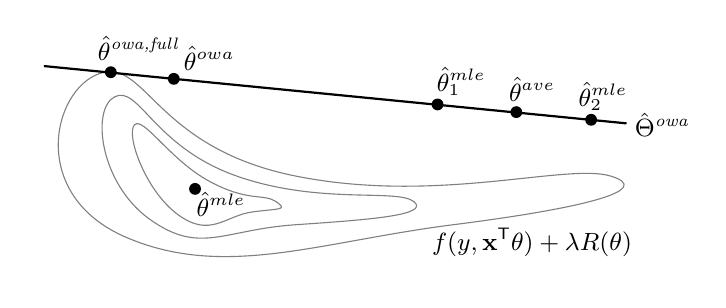
\begin{tikzpicture}
    [
    dot/.style = {minimum width=0.15cm,inner sep=0pt,line width=0pt,fill,circle,black,font=\small}
    , yscale=0.65
    ]
\small
\draw[gray] plot [smooth cycle,tension=1] coordinates {(-0.5,-0.75) (-1.05,1) (-0.1,-0.1) (0.75,-0.5) (0.45,-0.7) };
\draw[gray] plot [smooth cycle,tension=1] coordinates {(-0.85,-0.85) (-1.3,1.55) (0.25,0) (2.5,-0.5) (1,-0.95)};
\draw[gray] plot [smooth cycle,tension=1] coordinates {(-1.15,-1.2) (-1.5,2) (1,0) (5,0) (3,-0.95)};

\draw[thick] (-2.2,2.15) -- (5.2,1.03);

\node[dot] (wstar) at (-0.28,-0.25) {};
\node at (0.05,-0.55) {$\wmle$};

%\node[dot] (wstarproj) at (0.1,1.8) {};
%\draw (wstar) -- (wstarproj);
%\draw (0.07,1.65) -- (0.23,1.62) -- (0.26,1.78);

%\node[dot] (wavestar) at (4,0.5) {};
%\node                 at (4.5,0.3) {$\E\wave$};
\node[dot] (wave) at (3.8,1.25) {};
\node at (4.0,1.7) {$\wave$};
\node[dot] (wave) at (2.80,1.40) {};
\node at (3.1,1.85) {$\wmle_1$};
\node[dot] (wave) at (4.75,1.10) {};
\node at (4.9,1.55) {$\wmle_2$};
%\node[dot] (wave) at (3.8,1.25) {};

\node[dot] at (-1.35,2.03) {};
\node at (-1.0,2.5) {$\wowafull$};

\node[dot] at (-0.55,1.9) {};
\node at (-0.1,2.3) {$\wowa$};

\node at (4,-1.3) {$f(y,\trans\x\w)+\lambda R(\theta)$};
\node at (5.65,1.0) {$\W$};
\end{tikzpicture}
\vspace{-0.35in}
\caption{
    Our method performs a second round of optimization to find the best parameter vector in $\W$.
    %Since $\wave\in\W$, the estimator $\wowafull$ has higher empirical likelihood than $\wave$.
    Since $\W$ has low dimension, we can use relatively few data points in the second round of optimization to ensure that with high probability $\wowa$ has higher empirical likelihood than $\wave$.
    %Since $\W$ has low dimension, we can use relatively few data points in the second round of optimization to ensure that $\ltwo{\wowafull-\wowa}$ is small.
}
\label{fig:contour}
\end{figure}

Calculating the weights $\afull$ directly is infeasible because it requires access to the full dataset.
Fortunately, we do not need to consider all the data points for an accurate estimator.
The parameter space $\W$ is $m$-dimensional.
So intuitively, we only need $O(m)$ data points to solve the second optimization to our desired accuracy.
%(This intuition is formalized in Section \ref{sec:anal}.)
This intuition motivates the OWA estimator.
Let $\Zowa_i\subset Z_i$ be a set of $\nowa$ data points uniformly sampled from $Z_i$ without replacement,
and let $\Zowa$ be the union of the $\Zowa_i$s.
Then the OWA estimator is defined as
\begin{equation}
\wowa = \matW \ahat,
\end{equation}
where
\begin{equation}
\label{eq:ahat}
\ahat = \argmax_\alpha \sum _{(\x,y)\in \Zowa} f\left(y,\trans\x \matW \alpha \right)
+ \lambda R (\matW\alpha)
.
\end{equation}

Algorithm \ref{fig:alg2} shows the steps for efficiently computing $\wowa$.
In the first round, each machine calculates $\wmle_i$ independently and broadcasts the result to every other machine.
Since the parameter vector has $d$ dimensions and there are $m$ machines, a total of $O(md)$ bits are transmitted.
In the second round, each machine projects its local dataset $\Zowa_i$ onto the space $\W$.
These projected data points are then transmitted to a predesignated master machine.
The projected data points each have dimension $m$, so a total of $O(m^2\nowa)$ bits are transmitted.
The master machine now has all of the information to complete the optimization.
In total, $O(md + m^2\nowa)$ bits were transmitted.
When $d<m\nowa$, this is the same order of bits as the averaging estimator.

%\begin{algorithm}[t]
%\caption{Distributed calculation of $\wowa$}
%\label{alg:distributed}
%\begin{algorithmic}
%\State Round 1, each machine $i$ independently:
%\State ~~~~~loads dataset $Z_i$
%\State ~~~~~calculates $\wmle_i$
%\State ~~~~~broadcasts $\wmle_i$ to all other machines
%\State Round 2, each machine $i$ independently:
%\State ~~~~~constructs $\matW$
%\State ~~~~~randomly selects a dataset $\Zowa_i\subset Z_i$
%\State ~~~~~calculates $\Zproj_i=\{(\trans\x\matW,y) : (\x,y)\in\Zowa\}$
%\State ~~~~~broadcasts $\Zproj_i$ to a master machine
%\State The master calculates $\wowa$
%\end{algorithmic}
%\label{fig:alg2}
%\end{algorithm}

%\subsection{Implementation Tips}
%
Equations \ref{eq:afull} and \ref{eq:ahat} cannot be solved directly using off the shelf optimizers because existing optimizers do not support the non-standard regularization term $R(\matW\alpha)$.
In practice, it is sufficient to approximate this regularization by L2 regularization directly on the $\alpha$ vector:
\begin{equation}
\lambda R(\matW\alpha) \approx \lambda_2 \ltwo{\alpha}
.
\label{eq:approxreg}
\end{equation}
Intuitively, this is because even when we want the parameter vector $\w$ to be sparse (and so are regularizing by $R = $ the L1 norm), we have no reason to believe that the $\alpha$ vector should be sparse.
The desired sparsity is induced by the regularization when solving for $\wmle_i$s and maintained in any linear combination of the $\wmle_i$s.
The new $\lambda_2$ regularization parameter should be set by cross validation.
This will be a fast procedure, however, because there are few data points to optimize over,
and the L2 regularized problem is much easier to solve than the L1 problem.
With this minor modification, our distributed estimator can be implemented using any existing optimizer.
%Our experimental results in Section \ref{sec:exp} use this modified version of $\hat\alpha$.

%It is also important when performing the second round of optimization to not extend the parameter vector with an intercept term as is typically done.
%It is fine to do this for the first round as long as the intercepts also get scaled.

\section{RELATED WORK}
\label{sec:relwork}

Related work can be divided into two categories:
alternative estimators,
and bounds on the communication complexity of distributed learning.

\subsection{Alternative estimators}
\label{sec:alt}
The simplest and most popular communication-efficient estimator is the averaging estimator
\begin{equation}
\wave = \frac{1}{m}\sum_{i=1}^m \wmle_i
.
\end{equation}
Previous analysis of $\wave$ makes a number of limiting assumptions.
\cite{mcdonald2009efficient} analyze $\wave$ in the special case of L2 regularized maximum entropy models.
They provide tail bounds on $\ltwo{\wstar-\wave}$, showing that the variance $\ltwo{\E\wave-\wave}$ reduces as $O((nm)^{-1/2})$,
but they do not show a reduction in bias.
Their analysis uses a martingale technique that requires the radius of the dataset be independent of the size of the dataset.
This is a particularly limiting assumption as even the simple case of
normally-distributed data does not satisfy it.
\cite{zhang2012communication} provide a more general analysis showing that the mean squared error (MSE) $\E\ltwo{\wstar-\wave}{}^2$ decays as $O((nm)^{-1} + n^{-2})$.
This matches the optimal MSE of $\wmle$ whenever $m<n$.
Their analysis still requires a number of technical assumptions.
For example, they assume the parameter space $\Theta$ is bounded.
This assumption does not hold under the standard Bayesian interpretation of L2 regularization as a Gaussian prior of the parameter space.
They further make strong convexity and 8\emph{th} order smoothness assumptions which guarantee that $\wmle_i$ is a ``nearly unbiased estimator'' of $\wstar$.
%(As we will see in the next subsection,
%recently developed information theoretic bounds show these assumptions are required to show a reduction in MSE to the single machine rate.)
%All previous analysis of $\wave$ assumes that the likelihood $f$ is concave.
In Section \ref{sec:anal}, we provide a simpler analysis of $\wave$ that relaxes these assumptions.
In particular, our analysis does not require any quantities to be bounded or the likelihood to be concave.

Other research has focused on modifications to the $\wave$ estimator to reduce bias.
\cite{zinkevich2010parallelized} show that if the training sets partially overlap each other (instead of being disjoint), then the resulting estimator will have lower bias.
%The authors admit their analysis is ``highly technical.''
\cite{zhang2012communication} also provide a bootstrap average estimator,
which works as follows.
Let $r\in(0,1)$, and $Z_i^r$ be a bootstrap sample of $Z_i$ of size $rn$.
Then the bootstrap average estimator is
\begin{equation}
\wboot = \frac{\wave-r\waver}{1-r}
,
\end{equation}
where
\begin{equation}
\begin{aligned}
\waver &= \frac{1}{m}\sum_{i=1}^m \wmler_i
,
\\
\wmler_i &= \argmax_\w \sum_{(\x,y)\in Z_i^r} f(y,\trans\x\w) + \lambda R(\w)
.
%\\
%,
%\\
%\wboot & = \frac{\wave-r\waver}{1-r}
%.
\end{aligned}
\end{equation}
The intuition behind this estimator is to use the bootstrap sample to directly estimate and correct for the bias.
This estimator enjoys a MSE that decays as $O((nm)^{-1}+n^{-3})$ under similar assumptions as their analysis of $\wave$.
There are two main limitations to $\wboot$.
First, the optimal value of $r$ is not obvious and setting the parameter requires cross validation on the entire data set.
Our proposed $\wowa$ estimator has a similar parameter $\lambda_2$ that needs tuning,
but this tuning happens on a small fraction of the data and always with the L2 regularizer.
So properly tuning $\lambda_2$ is more efficient than $r$.
Second, performing a bootstrap on an unbiased estimator increases the variance.
This means that $\wboot$ could perform worse than $\wave$ on unbiased estimators.
Our $\wowa$ estimator, in contrast, will perform at least as well as $\wave$ with high probability as seen in Figure \ref{fig:contour}.
In Section \ref{sec:exp}, we show that our estimator has better empirical performance.

%An alternative definition of the $\wave$ estimator is
%\begin{equation}
%\wave = \argmin_\w \frac{1}{m}\sum_{i=1}^m \ltwo{\wmle_i-\w}^2
%\end{equation}
%It is easy to show that the two definitions are equivalent with standard calculus.

\cite{liu2014distributed} propose a more Bayesian approach inspired by \cite{merugu2003privacy}.
Instead of averaging the model's parameters,
they directly ``average the models'' with the following KL-average estimator:
\begin{equation}
\wkl = \argmin_\w \sum_{i=1}^m \kl[\bigg]{p(\cdot;\wmle_i)}{p(\cdot;\w)}
.
\end{equation}
The minimization is performed via a bootstrap sample from the smaller models.
This method has two main advantages.
First, it is robust to reparameterizations of the model.
Second, it is statistically optimal for the class of non-interactive optimization methods.
(We show in the next section that this optimality bound does not apply to our $\wowa$ estimator due to our semi-interactive setting.)
The main downside of the KL-average is that the minimization has a prohibitively high computational cost.
Let $n^{kl}$ be the size of the bootstrap sample.
Then the original implementation's MSE shrinks as $O((nm)^{-1}+(nn^{kl})^{-1})$.
This implies that the bootstrap procedure requires as many samples as the original problem to get a MSE that shrinks at the same rate as the averaging estimator.
\cite{han2016bootstrap} show a method to reduce this rate to $O((nm)^{-1}+(n^2n^{kl})^{-1})$ using control variates, but the procedure remains prohibitively expensive.
Their experiments show the procedure scaling only to datasets of size $nm\approx10^4$,
whereas our experiments involve a dataset of size $nm\approx10^8$.

Surprisingly, \cite{zhang2013divide} show that in the special case of kernel ridge regression,
a reduction in bias is not needed to have the MSE of $\wave$ decay at the optimal sequential rate.
By a careful choice of regularization parameter,
they cause $\wmle_i$ to have lower bias but higher variance,
so that the final estimate of $\wave$ has both reduced bias and variance.
%This suggests that once the proper regularization parameter is known,
%there is no need for a bias reduction at all.
This suggests that a merging procedure that reduces bias is not crucial to good performance if we set the regularization parameter correctly.
Typically there is a narrow range of good regularization parameters,
and finding a $\lambda$ in this range is expensive computationally.
We show experimentally in Section \ref{sec:exp} that our method has significantly reduced sensitivity to $\lambda$.
Therefore, it is computationally cheaper to find a good $\lambda$ for our method than for the other methods discussed in this section.

\subsection{Performance bounds}
\label{sec:bounds}

Performance bounds come in two flavors: statistical and information theoretic.
On the statistical side, \cite{liu2014distributed} show that for any non-interactive distributed estimator $\wq$,
the quantity $\ltwo{\wq-\wmle}{}^2$ decays as $\Omega(\gamma^2_\wstar \I^{-1}_\wstar/n^2)$.
Here $\gamma_\wstar$ is the statistical curvature of the model and $\I_\wstar$ is the Fisher information.
Furthermore, they show that $\wkl$ matches this bound.
This bound is not relevant for our $\wowa$ estimator because of our semi-interactive setting.
A crucial assumption of Liu and Ihler's analysis is that the merge function not depend on the data.
%Furthermore, we directly optimize $\ltwo{\wq-\wstar}^2$ which is a more useful quantity in practice.

\cite{shamir2014fundamental}, \cite{zhang2013information}, and \cite{garg2014communication} all provide information theoretic lower bounds on the sample complexity of non-interactive learning problems.
As above, however, their results are not applicable in our semi-interactive setting.
%provides general information theoretic bounds for what he terms learning with information constraints.
%As a special case of Shamir's analysis is the non-interactive communication model where $q$ does not depend on the data.
%When $q$ is allowed to depend on the data, his model no longer applies.
There is one information theoretic lower bound that does apply to us.
Let the true parameter vector $\wstar$ be $k$-sparse.
That is, $\lzero{\wstar} \le k$.
%Then \cite{zhang2013information} showed that at least $\Omega(mk/\log m)$ bits of communication are required in the non-interactive setting,
%and \cite{garg2014communication} improved this lower bound to $\Omega(mk)$.
Surprisingly, \cite{braverman2015communication} show that the minimax optimal error rate for least squares regression requires $\Omega(m\cdot\min\{n,d\})$ bits of communication (independent of $k$) even in the fully interactive setting.
This is important because sparsity does not reduce the amount of communication required, and this bound does apply in our setting.

\section{ANALYSIS}
\label{sec:anal}

In this section, we analyze the statistical performance of our $\wowa$ estimator.
As part of the analysis, we provide a novel proof of the statistical performance of $\wave$ with an easier to interpret constant factor.
Our analysis is simpler and more general than previous analyses of distributed estimators.
In particular, we do not assume that any random variables are bounded
or that our likelihood function is concave.

\subsection{Conditions}

The only condition of our analysis is that the estimation error has sub-Gaussian tails.
We first state this condition formally,
then explain why this condition is mild.

\begin{defn}
We say that a random vector $\x$ is \emph{sub-Gaussian} with variance proxy $\sigma^2$ if it obeys the following concentration bound.
Let $t>0$, then with probability at least $1-\exp(-\sigma^2t^2/2)$,
%\begin{equation}
$
\ltwo{\x} < t
$.
%\end{equation}
\end{defn}

Note in particular that if $\x$ is a Gaussian random vector with mean $\mu$ and covariance $\Sigma$,
then $\Sigma^{1/2}(\x-\mu)$ is sub-Gaussian with $\sigma^2=1$.
Sub-Gaussian random vectors have recently become an important tool in the analysis of high dimensional statistics.
\cite{vershynin2010introduction} provides an accessible tutorial of these results.
We now state our condition.

\newtheorem*{sgt}{The Sub-Gaussian Tail (SGT) Condition}
\begin{sgt}
Let $\theta$ be an estimator trained on $n$ data points.
%Let $t>0$ and $\sigma^2$ be a constant called the \emph{variance proxy}.
%Then with probability at least $1-\exp(-\sigma^2t^2/2)$,
%\begin{equation}
%%\ltwobig{\I^{-1/2}_\wstar(\wmle_i-\wstar)} < \frac{t}{\sqrt n}
%%\sqrt n \ltwobig{\I^{-1/2}_\wstar(\wmle_i-\E\wmle_i)} < t
%\sqrt n \ltwobig{\I^{-1/2}_\wstar(\theta-\E\theta)} < t
%,
%\end{equation}
Then the random vector
\begin{equation}
%\Delta_\theta = \sqrt{n}\ltwo{\I^{1/2}_\wstar(\theta-\E\theta)}
\Delta_\theta = \sqrt{n}{\I^{1/2}_\wstar(\theta-\E\theta)}
\end{equation}
is sub-Gaussian for some $\sigma^2$.
Above, $\I_\wstar$ is the positive definite Fisher information matrix at the parameter vector's true value $\wstar$.
%which is sub-Gaussian by assumption.
\end{sgt}

%Sub-Gaussian distributions have recently become an important tool in the analysis of high dimensional statistics.
%\cite{vershynin2010introduction} provides an accessible tutorial of these results.

The SGT condition is mild and known to hold in many situations of interest.
In the asymptotic regime when $n\to\infty$,
very strong results are known.
%this condition is known as root-$n$ consistency.
%In this case,
%The error $\Delta_\theta$ is exactly Gaussian.
Theorem 7.5.2 of \cite{lehmann1999elements} is a simple example that shows $\Delta_\theta$ is an isotropic centered Gaussian
(and hence sub-Gaussian).
Lehman's theorem requires only that $f$ be three times differentiable,
the data points be i.i.d.,
and some mild identifiability conditions.
More sophisticated analyses show that the SGT Condition holds very generally.
For example \cite{spokoiny2012parametricestimation} shows that $\Delta_\w$ is normally distributed even when the data points are correlated.

Similar results hold in the non-asymptotic case $n<\infty$,
but known results are less strong.
Most non-asymptotic results of this form require that the data points also be sub-Gaussian.
For example, \cite{negahban2009unified} considers the case when the data points are sub-Gaussian, the likelihood satisfies a ``restricted strong convexity condition,'' and the regularizer is decomposable.
More recently, \cite{sivakumar2015beyond} showed the SGT Condition holds when the data are only sub-exponential.
The strongest non-asymptotic results on the estimation error known to the authors are due to \cite{spokoiny2012parametricestimation}.
Spokoiny does not require any conditions on the data,
but shows that the SGT Condition is satisfied only up to $t < O(n)$.

Our analysis below requires that $\wmle_i$ satisfy the SGT Condition.
This is strictly more general than the conditions in previous work.
\cite{zhang2012communication} for example require that the parameter space $\Theta$ be bounded (in addition to other moment conditions).
A bounded parameter space automatically implies that $\wmle_i$ satisfies the SGT Condition because every bounded random variable is sub-Gaussian by definition.

%In conclusion,
%there are many ways to verify that the SGT Condition holds.
%Pick whichever one suits your problem.

\subsection{Analysis of $\wave$}

We provide a simple bound that shows that averaging improves the variance,
but not the bias of an estimator.
Similar bounds are well known (see Section \ref{sec:alt}),
but our analysis has the following advantages:
It requires fewer assumptions, has a simpler proof, and has an easy to interpret constant factor.

\begin{theorem}
\label{thm:wave}
Assume $\wmle_i$ satisfies the SGT Condition.
Let $t>0$.
Then with probability at least $1-\exp(-t)$,
\begin{equation}
\ltwo{\wstar-\wave} \le \ltwo{\wstar-\E\wmle_i} + \sqrt\frac{v_t}{mn}
\end{equation}
where
\begin{equation}
v_t =
\sigma^2
\left(
\tr{\I^{-1}_{\wstar}}
+ 2\sqrt{\tr \left({\I^{-2}_{\wstar}}\right)t}
+ 2\ltwo{\I^{-1}_{\wstar}}t
\right)
\label{eq:vt}
\end{equation}
\end{theorem}


Note that this reduction in variance is essentially optimal.
If we assume that $\wmle$ satisfies the SGT condition
(in most cases this follows from $\wmle_i$ satisfying the SGT condition),
then we are assuming that the variance of $\wmle$ reduces at the same $O(1/\sqrt{mn})$ rate.
%By an argument similar to Equations \ref{eq:var1}-\ref{eq:var2},
%we can show that the variance of the maximum likelihood estimator trained on all of the data is
%\begin{equation}
%\wmle - \E\wmle \sim \frac{1}{\sqrt{mn}} \normal{\zero}{\I^{-1}_{\wmle}}
%\label{eq:var3}
%\end{equation}
%The only difference between Equations \ref{eq:var2} and \ref{eq:var3} is the location of the Fisher information matrix.

\subsection {Analysis of $\wowa$}

Unlike the $\wave$ estimator,
$\wowa$ reduces both bias and variance.
The $m$ and $\nowa$ parameters act as ``knobs'' that let us trade off lower statistical error for higher communication cost.
%In particular, the number of machines $m$ acts as a ``knob'' that lets us
%In this section, we present one main theorem and two supporting lemmas.
%We begin our discussion with the following informal theorem statement.
Before we present the formal analysis,
we present a motivating informal analysis.

\subsubsection{Informal Analysis}
%The following theorem statement ignores constant factors.
%Our main result can be stated with the following informal theorem.
%We first state our main result informally,
%then describe its implications.
Our main result is captured in the following theorem.
\newtheorem*{theoreminf}{Theorem 2 (Informal)}
\begin{theoreminf}
With high probability, we have that
\begin{equation}
\nonumber
\ltwo{\wstar-\wowa}
\le
O\!\left(\!\!
    \sqrt{\frac{1}{m\nowa}}
    +
    \sqrt{\left(1-\frac{m}{d}\right)}\ltwo{\wstar-\wave}
\right)
\label{eq:informal}
\end{equation}
\label{thm:informal}
\end{theoreminf}
\vspace{-0.25in}
The rightmost term above captures the error of the optimal parameter vector constrained to $\W$.
That is, if
\begin{equation}
\wowastar = \argmin_{\w\in\W} \int_{\X\times\Y} \left(f(y,\trans\x\w) + \lambda R(\w)\right) d(\x,y)
,
\end{equation}
then the rightmost term is the error of $\ltwo{\wstar-\wowastar}$.
Clearly, as $m \to d$, the space $\W \to \Theta$, so $\wowastar\to\wstar$, and $\ltwo{\wstar-\wowastar}\to 0$.

The leftmost term above captures the error due to using only $\nowa$ data points in the second round of optimization.
That is, the leftmost term captures the error $\ltwo{\wowa-\wowastar}$.
As $\nowa\to n$, this error approaches the error of the oracle estimator trained on all the data $\ltwo{\wstar-\wmle}=O(1/\sqrt{mn})$.
By increasing $m$ and $\nowa$ our estimator is closer to the sequential oracle
at the expense of a higher communication cost.

\subsubsection{Formal Analysis}

In this section we give a version of Theorem 2 with explicit constant factors.
The proof is divided into two lemmas,
which we present first because they introduce important notation.
In the first lemma we bound the distance $\ltwo{\wstar-\proj{\W}\wstar}$,
where $\proj{\W}$ denotes the orthogonal projection onto $\W$.
In the second lemma, we show that $\proj{\W}\wstar \approx \wowa$.

%%%%%%%%%%%%%%%%%%%%%%%%%%%%%%%%%%%%%%%%

\begin{lemma}
\label{lem:proj}
Assume $\wmle_i$ satisfies the SGT condition.
Let $t>0$ and
\begin{equation}
\delta = 1-\exp((d-m)(-t+\ln(t+1)))
.
\label{eq:delta}
\end{equation}
Then we have that with probability at least $\delta$,
\begin{equation}
\ltwo{\wstar-\proj\W\wstar}
\le
(t+1)\sqrt{\frac\smin\smax\left(1-\frac{m}{d}\right)}\ltwo{\wstar - \wave}
\end{equation}
where $\smin$ and $\smax$ are the minimum and maximum eigenvalues of $\I_\wstar^{-1}$.
\end{lemma}

The proof uses standard properties of projection matrices with sub-Gaussian columns.
Due to space limitations, it is included in Appendix A of the supplement.
%
%%%%%%%%%%%%%%%%%%%%%%%%%%%%%%%%%%%%%%%%
%
%Our next lemma bounds the error of $\wowa$ in terms of the error of other estimators whose error we know.
Our next lemma shows that $\proj{\W}\wstar \approx \wowa$.
%We introduce the following notation.

\begin{lemma}
Let $\qhi,\qlo : \mathbb{R}^+ \to \mathbb{R}^+$ be monotonically increasing functions such that for all points $\w\in\Theta$,
\begin{align}
F(\wstar) - F(\w) &\ge \qlo \left( \ltwo {\wstar - \w} \right)
,
\\
F(\wstar) - F(\w) &\le \qhi \left( \ltwo {\wstar - \w} \right)
.
\end{align}
Then we have that
\begin{equation}
\begin{aligned}
\ltwo {\wstar-\wowa}
&\le
\ltwo{\wowastar-\wowa}
\\
&~~~+
\qlo^{-1} \left(
    \qhi \left( \ltwo {\wstar - \proj\W\wstar} \right)
\right)
.
\label{eq:lemma2res}
\end{aligned}
\end{equation}
\end{lemma}

The proof of Lemma 2 is a straightforward application of the triangle inequality.
It is contained in Appendix B of the supplement.
We are now ready to state a formal version of the informal Theorem 2.

%%%%%%%%%%%%%%%%%%%%%%%%%%%%%%%%%%%%%%%%

\begin{figure*}[t]
%\begin{tikzpicture}
%\node at (0,2) {};
%\node at (0,-2) {};
%\begin{tabular}{ccc}
  %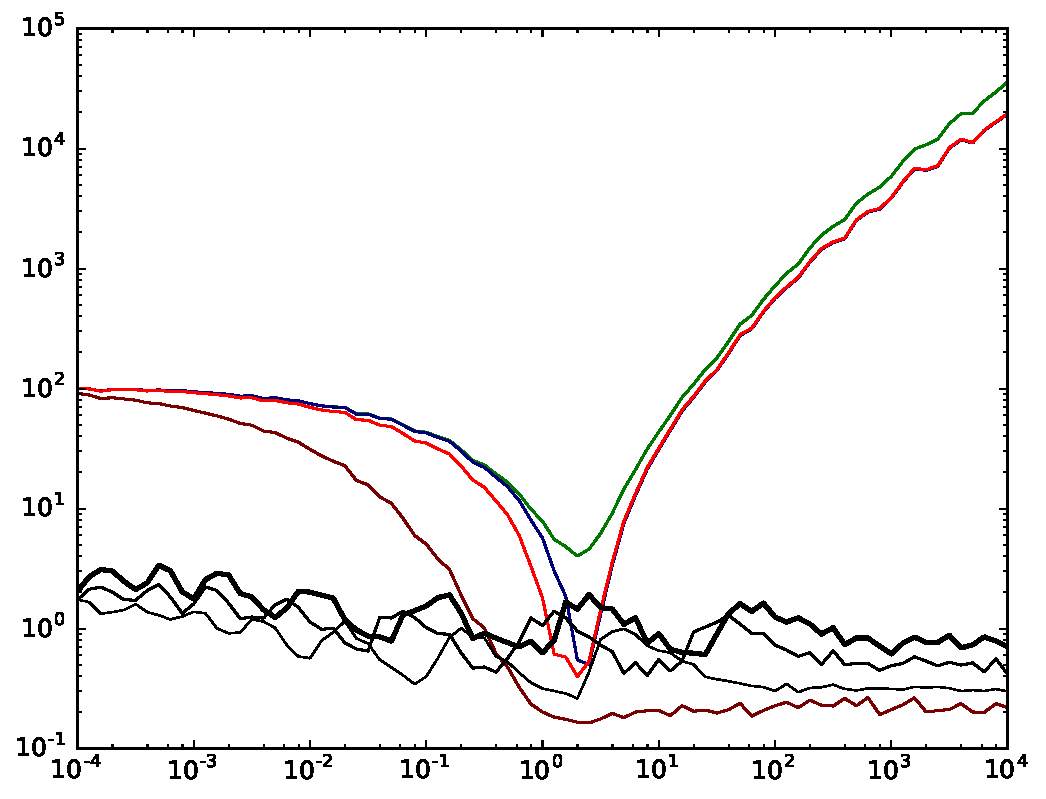
\includegraphics[width=0.3\textwidth]{img/logl2-star-logl2-auto-normal-log-1000-100-20}
%& 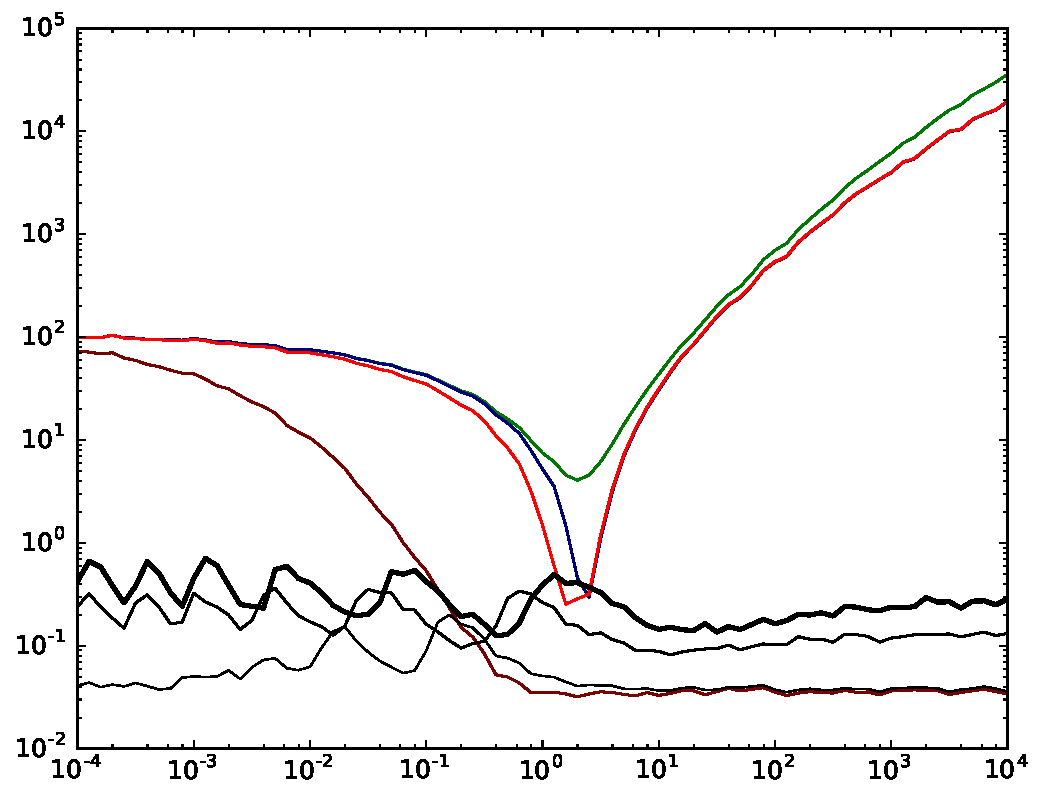
\includegraphics[width=0.3\textwidth]{img/logl2-star-logl2-auto-normal-log-1000-100-100}
%& 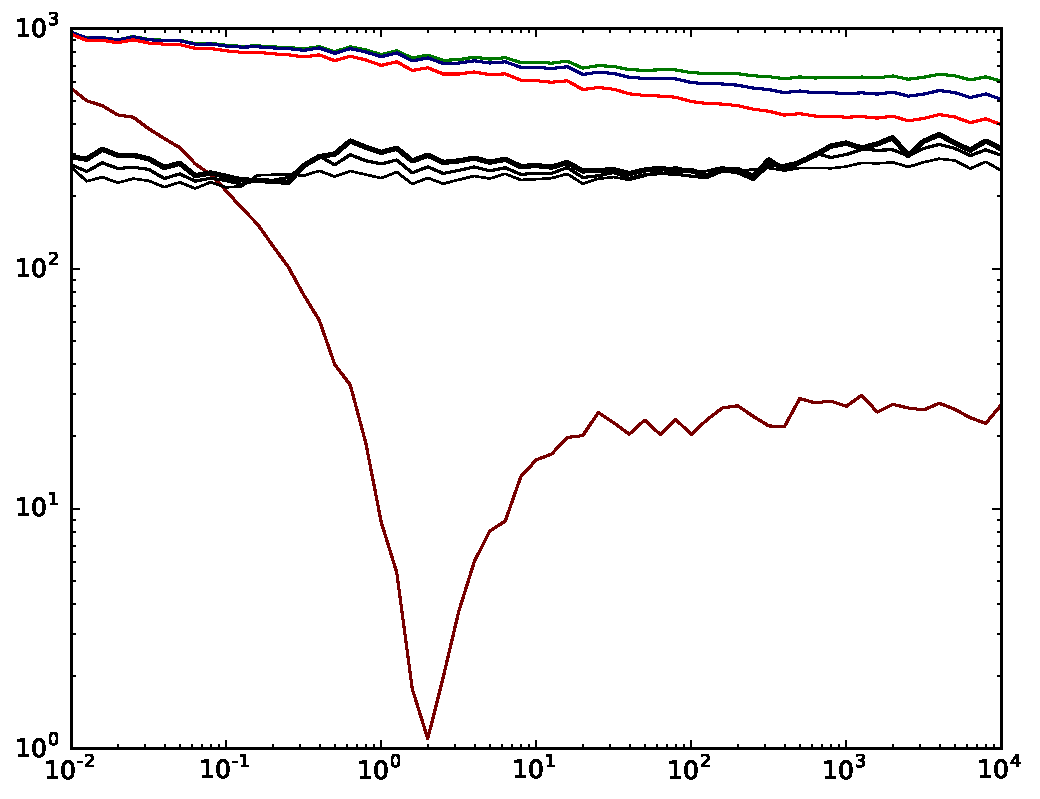
\includegraphics[width=0.3\textwidth]{img/logl2-star-logl2-auto-normal-log-1000-1000-100}
%\\
  %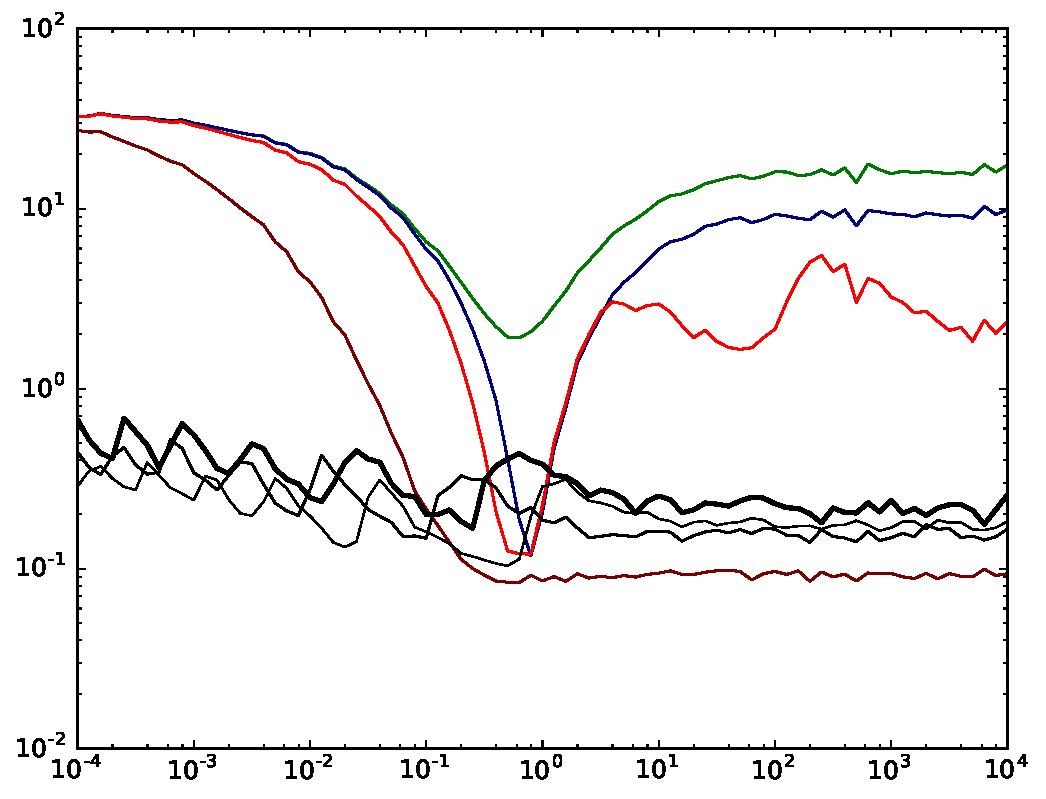
\includegraphics[width=0.3\textwidth]{img/logl2-star-logl2-auto-uniform-log-1000-100-20}
%& \includegraphics[width=0.3\textwidth]{img/logl2-star-logl2-auto-uniform-log-1000-100-100}
%& 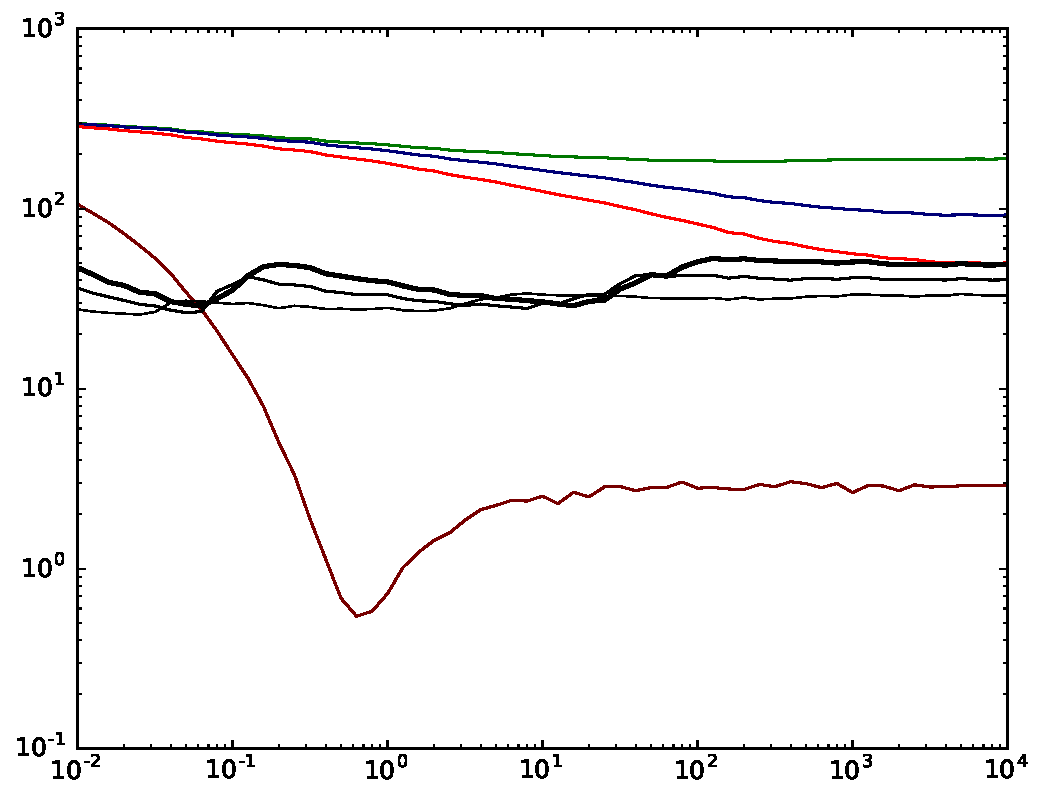
\includegraphics[width=0.3\textwidth]{img/logl2-star-logl2-auto-uniform-log-1000-1000-100}
%\\
  %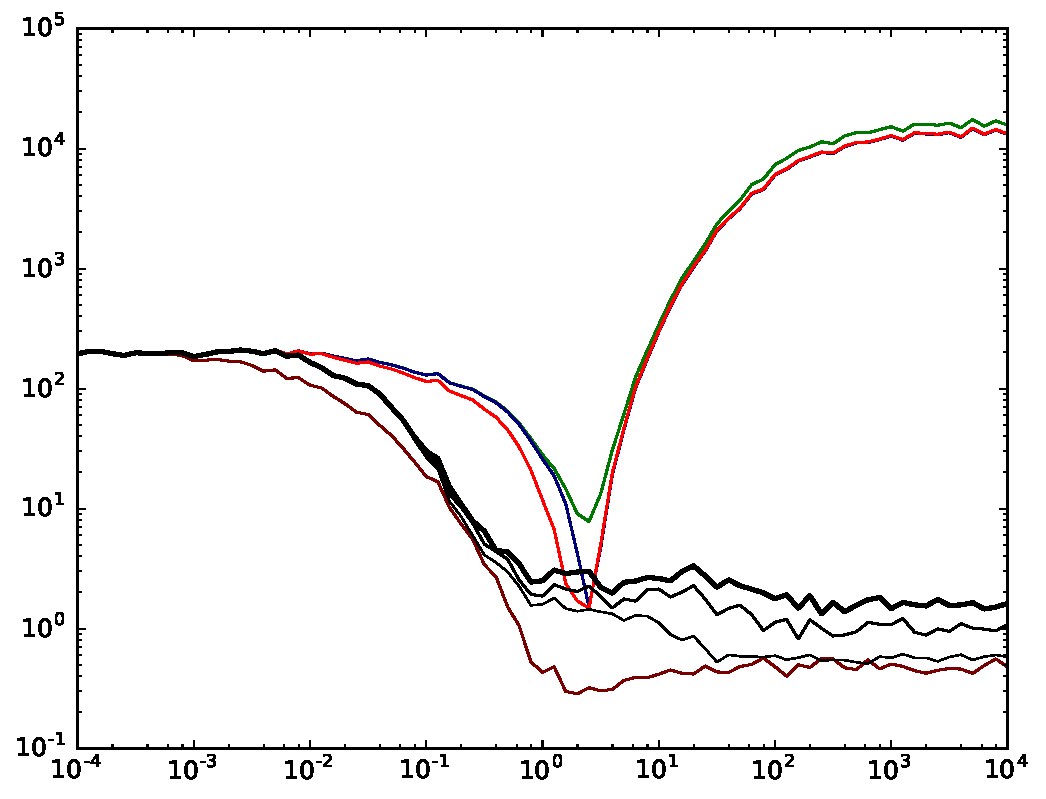
\includegraphics[width=0.3\textwidth]{img/logl1-star-logl2-autoreg-laplace-log-1000-100-20}
%& 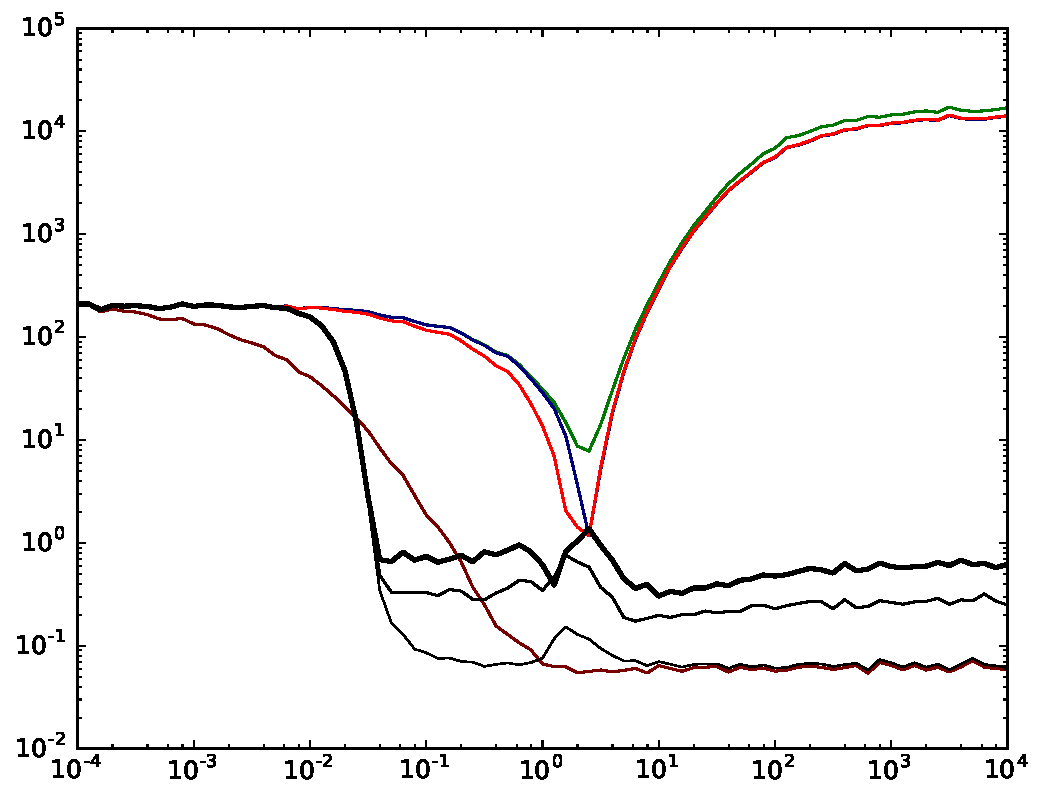
\includegraphics[width=0.3\textwidth]{img/logl1-star-logl2-auto-laplace-log-1000-100-100}
%& 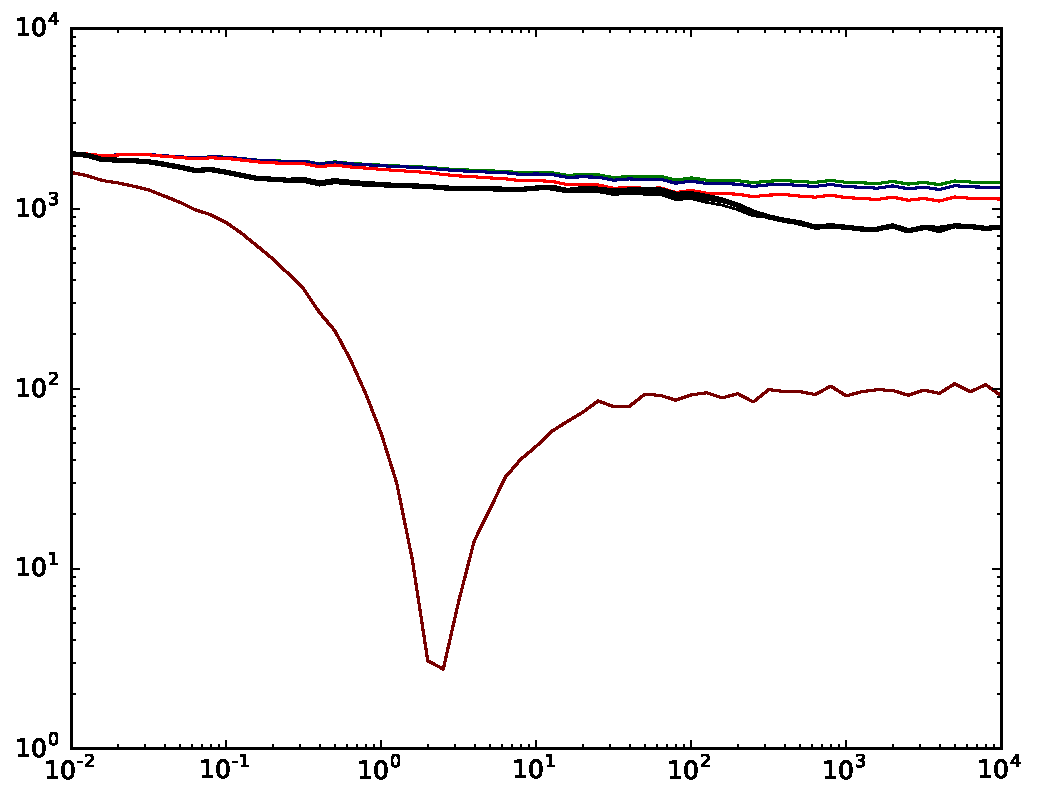
\includegraphics[width=0.3\textwidth]{img/logl1-star-logl2-auto-laplace-log-1000-1000-100}
%\\
  %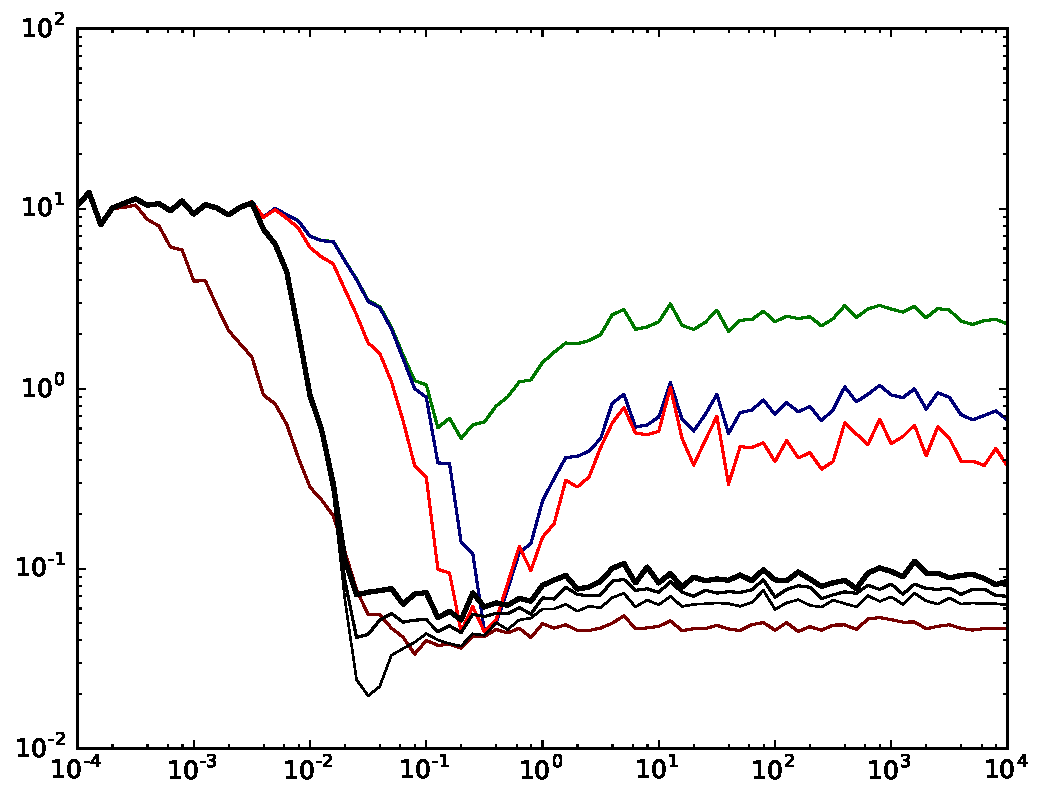
\includegraphics[width=0.3\textwidth]{img/logl1-star-logl2-autoreg-spike-log-1000-100-20}
%& 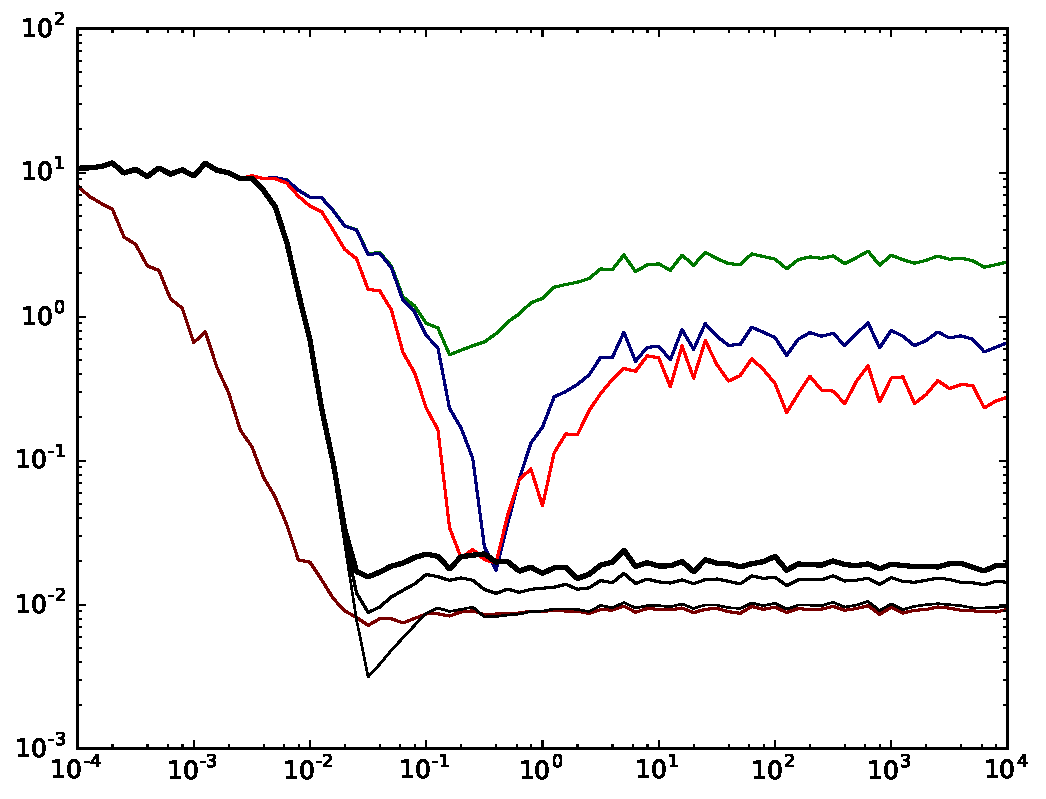
\includegraphics[width=0.3\textwidth]{img/logl1-star-logl2-auto-spike-log-1000-100-100}
%& 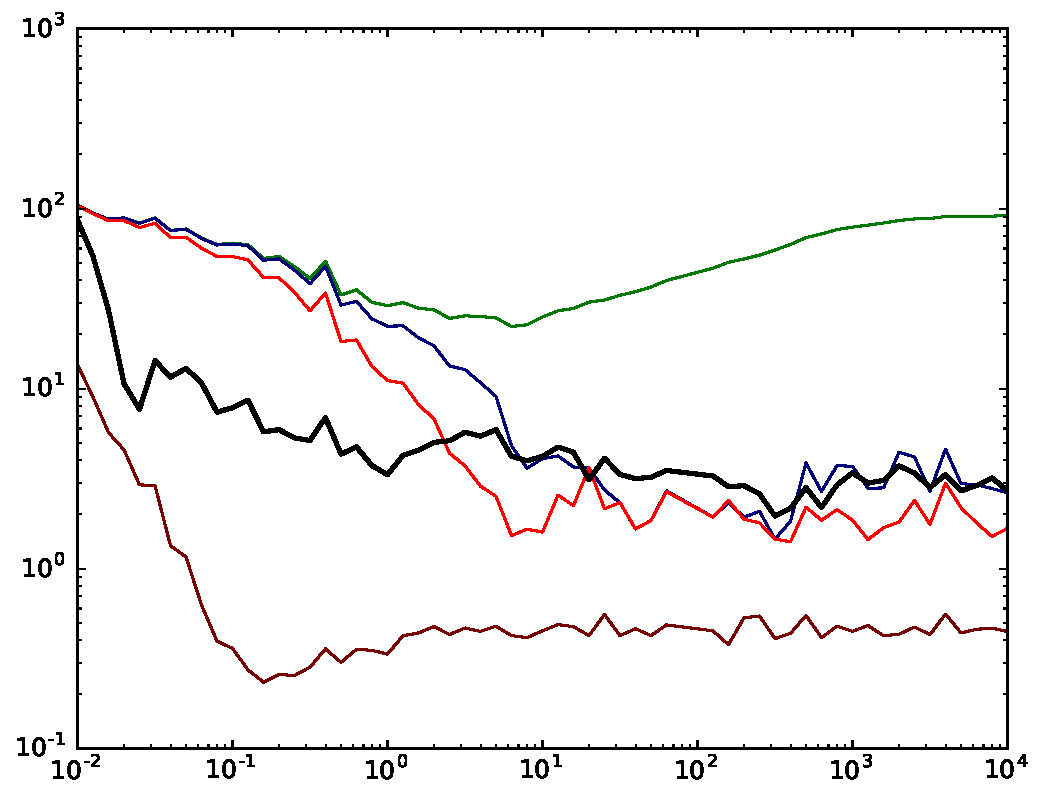
\includegraphics[width=0.3\textwidth]{img/logl1-star-logl2-auto-spike-log-1000-1000-100}
%\end{tabular}
%\end{tikzpicture}
\plots{
\newcommand{\mklambdaplot}[3]{
\begin{tikzpicture}
    [ yscale=0.8
    ]
\tiny
#3
\begin{axis}
    [ width=0.35\textwidth
    , xmode=log
    , ymode=log
    , xmin=10^-4
    , xmax=10^4
    , xtick={0.0001,0.01,1,100,10000}
    , enlarge y limits=0
#2
    ]
\addplot[black,no marks] table [x index=3,y index=5] {#1};
\addplot[brown,no marks] table [x index=3,y index=7] {#1};
\addplot[blue,no marks] table [x index=3,y index=9] {#1};
\addplot[red,thick,no marks] table [x index=3,y index=17] {#1};
\addplot[darkgreen,very thick,no marks] table [x index=3,y index=55] {#1};
\addplot[dotted,darkgreen,very thick,no marks] table [x index=3,y index=56] {#1};
\addplot[darkgreen,thin,no marks] table [x index=3,y index=56] {#1};
%\addplot[thick,red,no marks] table [x=n,y=bootll] {dat/kdd-scaling.dat};
%\addplot[very thick,darkgreen,no marks] table [x=n,y=owall] {dat/kdd-scaling.dat};
\end{axis}
%\node at (2.2,-0.8) {\small regularization strength ($\lambda$)};
\end{tikzpicture}
}
\begin{tabular}{cccc}
& $d=100,m=20$
& $d=100,m=100$
& $d=1000,m=100$
\\
{\small\rotatebox{90}{\hspace{0.05cm}squared error $\ltwo{\wstar-\w}^2$}}
&\hspace{-0.5cm}\mklambdaplot
    {dat/logl1-star-logl2-autoreg-spike-log-1000-100-20.pdf.csv}
    {,ymin=10^-2,ymax=10^2,ytick={0.01,0.1,1,10,100}}{
    \node at (2,2.4) {\textcolor{brown}{$\wmle_i$}};
    \draw[->,brown] (2,2.3) -- (2.1,2);
    \node at (3.5,1.95) {\textcolor{blue}{$\wave$}};
    \draw[->,blue] (3.5,1.9) -- (3.55,1.75);
    \node at (4,1.1) {\textcolor{red}{$\wboot$}};
    \draw[->,thick,red] (3.8,1.3) -- (3.75,1.45);
    \node at (0.5,1.85) {$\wmle$};
    \draw[->] (0.5,2.0) -- (0.6,2.2);
    \node at (0.7,0.9) {\textcolor{darkgreen}{$\wowa$}};
    \draw[->,thick,darkgreen] (0.9,0.8) -- (1.2,0.8);
    \node at (0.6,0.4) {\textcolor{darkgreen}{$\wowafull$}};
    \draw[->,thick,dotted,darkgreen] (0.9,0.3) -- (1.2,0.3);
    \draw[->,very thin,darkgreen] (0.9,0.3) -- (1.2,0.3);
    }
&\hspace{-0.5cm}\mklambdaplot
    {dat/logl1-star-logl2-auto-spike-log-1000-100-100.pdf.csv}
    {,ymin=10^-3,ymax=10^2,ytick={0.001,0.01,0.1,1,10,100}}
    {}
&\hspace{-0.5cm}\mklambdaplot
    {dat/logl1-star-logl2-auto-spike-log-1000-1000-100.pdf.csv}
    {,ymin=10^-1,ymax=10^3,ytick={0.1,1,10,100,1000}}
    {}
\\
& \hspace{0.2cm} {\small regularization strength ($\lambda$)}
&
&
\end{tabular}
}
\caption{
    OWA is robust to the regularization strength.
    Surprisingly, additional regularization introduced by OWA lets it outperform the oracle estimator $\wmle$ in some cases.
    Our theory states that as $m\to d$, $\wowa\to\wmle$.
    This is confirmed in the middle experiment.
    In the leftmost experiment, $m<d$, but $\wowa$ still behaves similarly to $\wmle$.
    In the rightmost experiment, $\wowa$ has similar performance as $\wave$ and $\wboot$ but is less sensitive to $\lambda$.
    }
\label{fig:lambda}
\end{figure*}

%%%%%%%%%%%%%%%%%%%%%%%%%%%%%%%%%%%%%%%%

\newtheorem*{theoremformal}{Theorem 2 (Formal)}
\begin{theoremformal}
Assume that $\wmle_i$ and $\alpha$ satisfy the SGT condition.
Let $t>0$ and
\begin{equation}
%\delta = 1-\exp((d-m)(-t+\ln(t+1)))
\delta = (1-\exp((d-m)(-t+\ln(t+1))))(1-\exp(-t))
.
\end{equation}
Then, with probability at least $\delta$,
\begin{equation}
\begin{aligned}
&\ltwo{\wstar-\wowa}
\\
&\le
%\ltwo{\wowastar-\wowa}
\ltwo{\wowastar-\E\wowa}
+ \sqrt{\frac{v_t}{m\nowa}}
\\
&+
\qlo^{-1}\bigg(\qhi\bigg((t+1)\sqrt{\frac{\smin}{\smax}\left(1-\frac{m}{d}\right)}\ltwo{\wstar-\wave}\bigg)\bigg)
\end{aligned}
\end{equation}
\end{theoremformal}

\begin{proof}
Bound the left term of Equation \ref{eq:lemma2res} using the procedure we used for Theorem 1.
Then use Lemma 1 to bound $\ltwo{\wstar-\proj\W\wstar}$ in the right term.
%Then use Lemma 1 to bound the rightmost term.
\end{proof}

\newpage

%There are two differences between the formal and informal version of Theorem 2 worth highlighting.
Notice that the formal version of Theorem 2 contains the term $\ltwo{\wowastar-\E\wowa}$, which does not appear in the informal version.
This is the bias of the second round of optimization in the subspace $\Wowa$ due to $\nowa$ being finite.
This bias will be less than the bias of the full problem because $\Wowa\subset\Theta$.
As $m\to\infty$, $\wowastar\to\wstar$ and $\E\wowa\to\W\wmle$, so $\ltwo{\wowastar-\E\wowa}\to\ltwo{\wstar-\E\wmle}$.
%Furthermore, this bias will reduce at the rate of $O(1/\sqrt{m\nowa})$ under standard assumptions.
%The next difference is the application of the functions $\qlo$ and $\qhi$.

\section{EXPERIMENTS}
\label{sec:exp}

We evaluate OWA on two logistic regression tasks.
The first task uses synthetic data.
The second task uses real world ad-click data from the Tencent search engine.
In each experiment, we compare our $\wowa$ estimator with four baseline estimators:
the naive estimator using the data from only a single machine $\wmle_i$;
the averaging estimator $\wave$;
the bootstrap estimator $\wboot$;
and the oracle estimator of all data trained on a single machine $\wmle$.
The $\wboot$ estimator has a parameter $r$ that needs to be tuned.
%We make an effort to present the $\wboot$ estimator in the best light possible.
In all experiments we evaluate $\wboot$ with $r \in \{0.005,0.01,0.02,0.04,0.1,0.2\}$,
which is a set recommended in the original paper \citep{zhang2012communication},
and then report only the value of $r$ with highest true likelihood.
Thus we are reporting an overly optimistic estimate of the performance of $\wboot$,
and as we shall see our estimator $\wowa$ still tends to perform better.

\subsection{Synthetic Data}

\begin{figure*}[t]
%\begin{tikzpicture}
%\begin{tabular}{ccc}
  %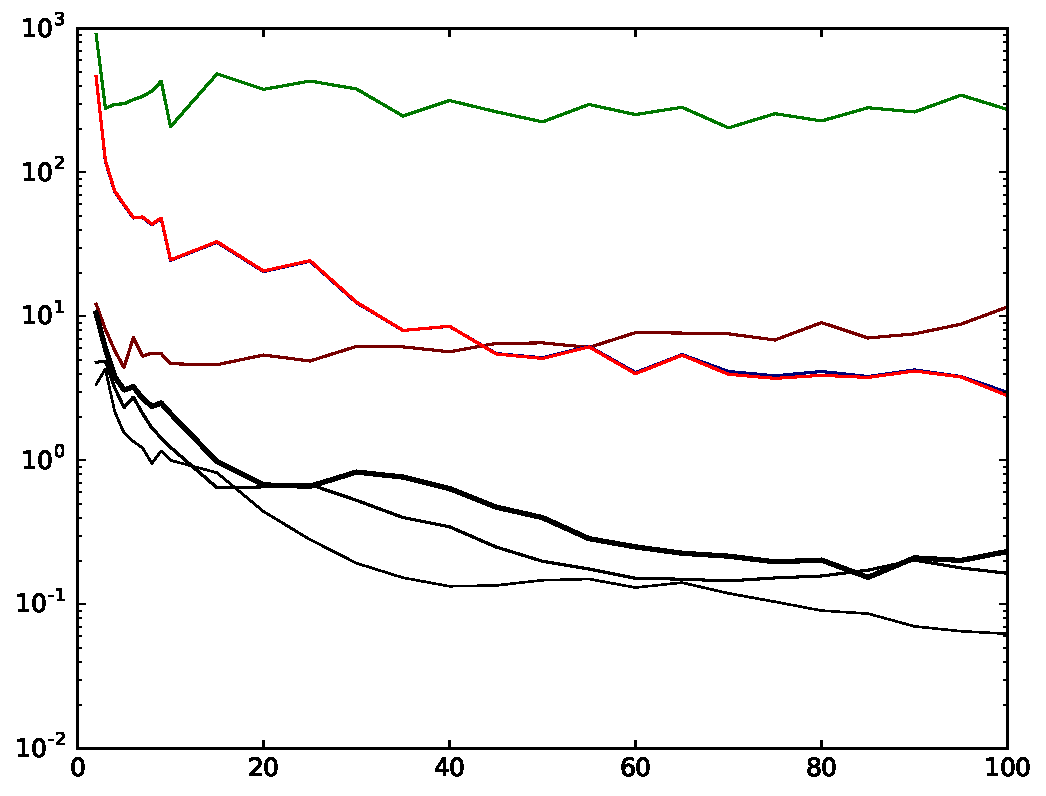
\includegraphics[width=0.3\textwidth]{img/logl2-auto-logl2-auto-normal-log-1000-100-star.pdf}
%& 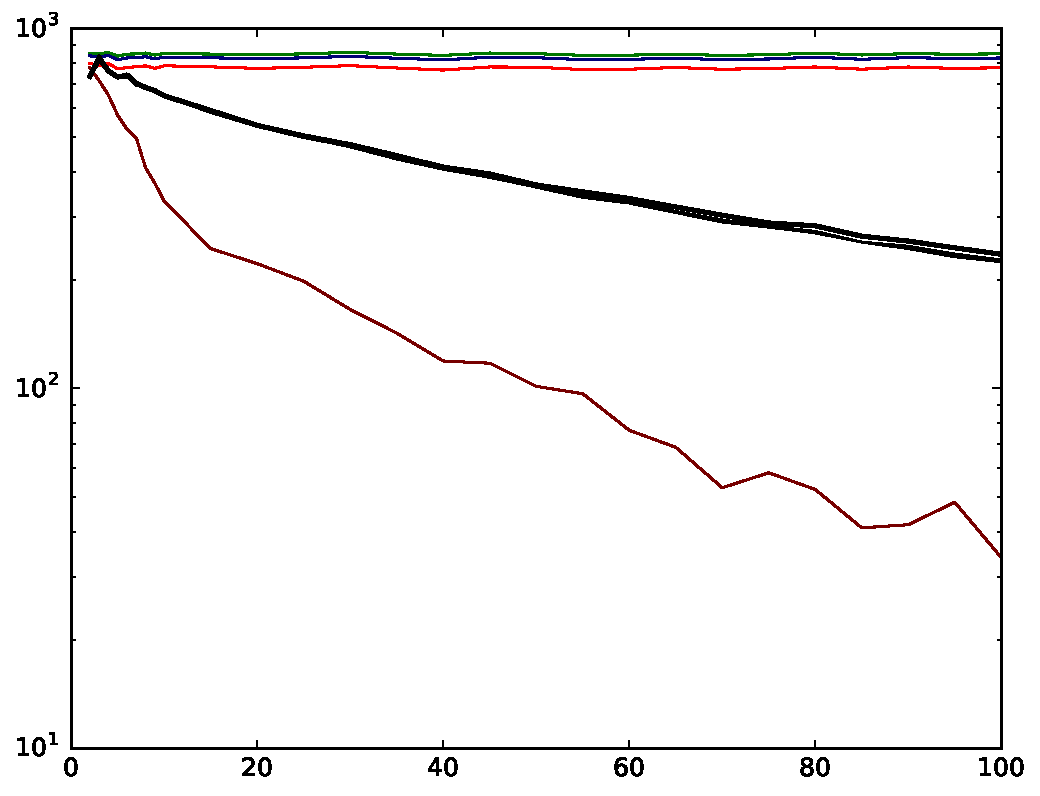
\includegraphics[width=0.3\textwidth]{img/logl2-auto-logl2-auto-normal-log-1000-1000-star.pdf}
%& 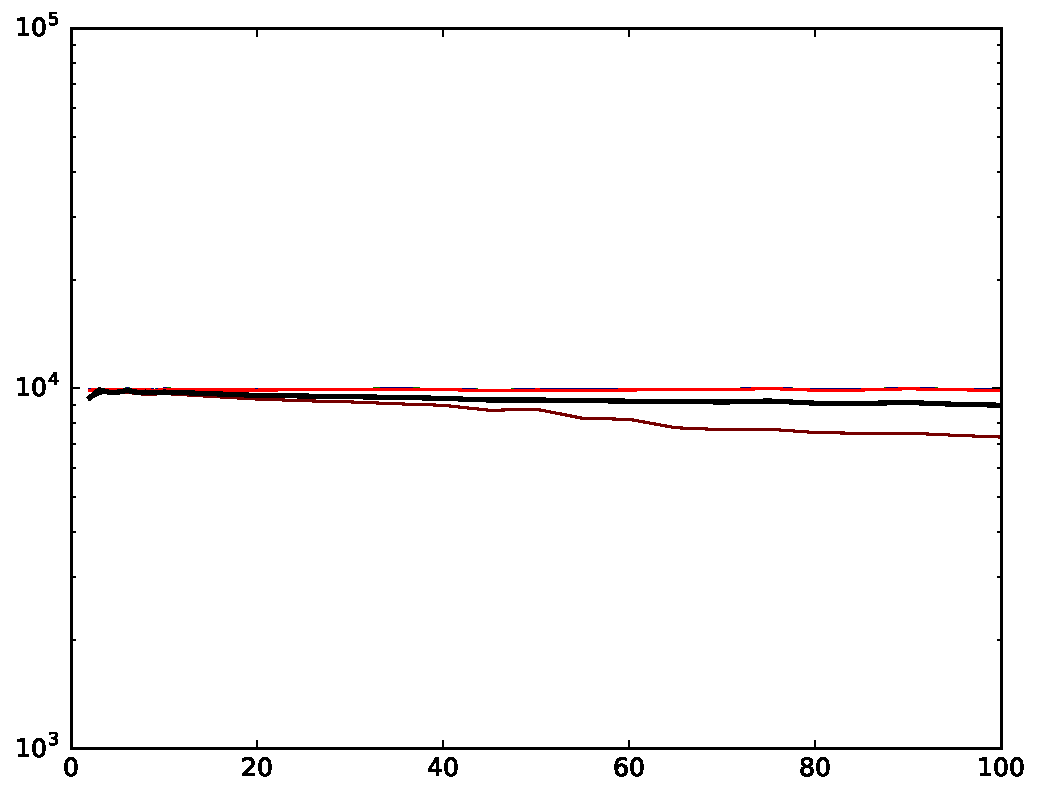
\includegraphics[width=0.3\textwidth]{img/logl2-auto-logl2-auto-normal-log-1000-10000-star.pdf}
%\\
  %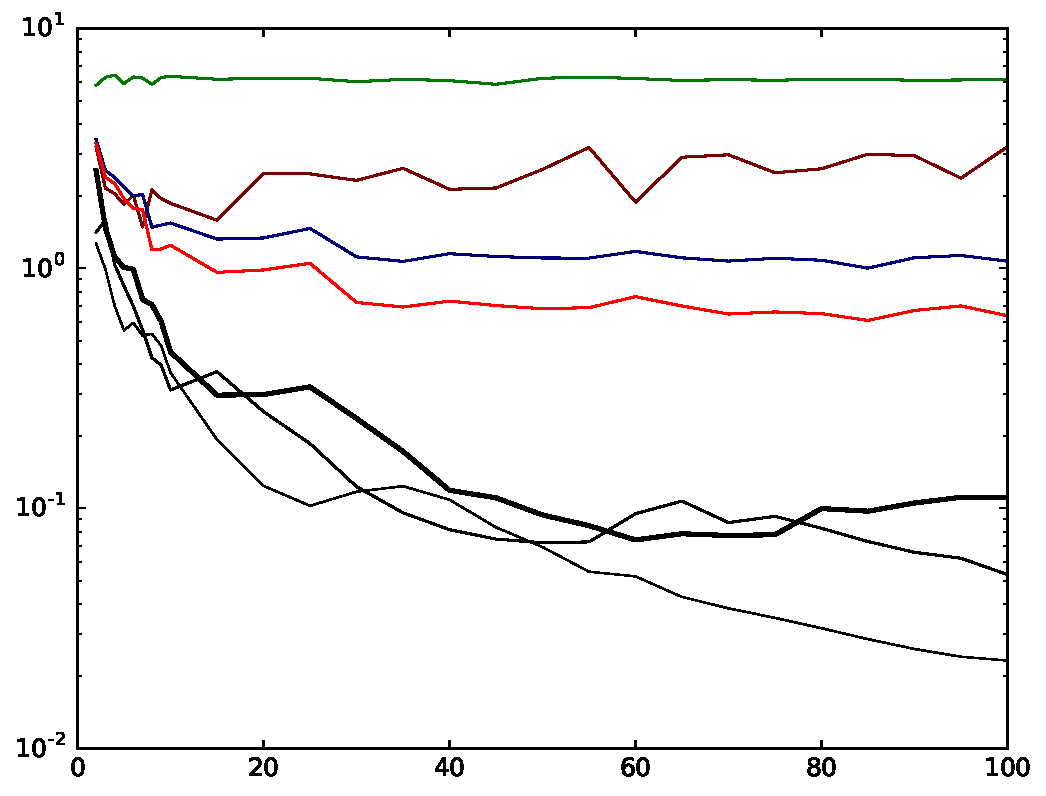
\includegraphics[width=0.3\textwidth]{img/logl2-auto-logl2-auto-uniform-log-1000-100-star.pdf}
%& 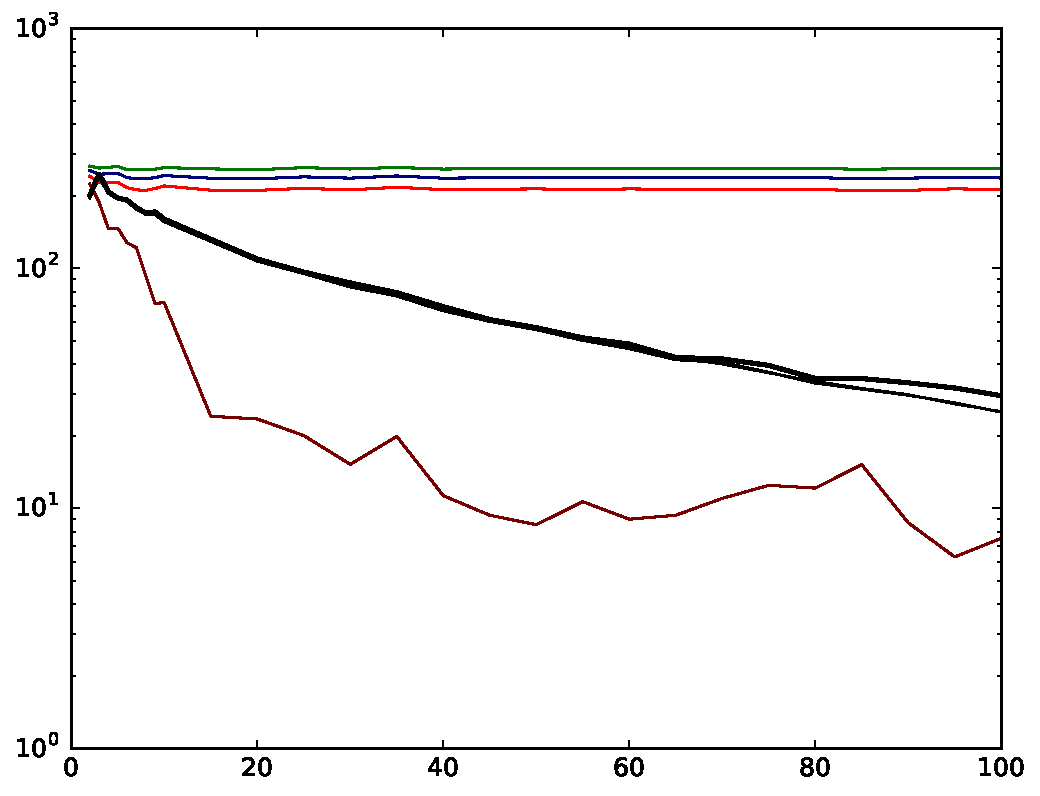
\includegraphics[width=0.3\textwidth]{img/logl2-auto-logl2-auto-uniform-log-1000-1000-star.pdf}
%& 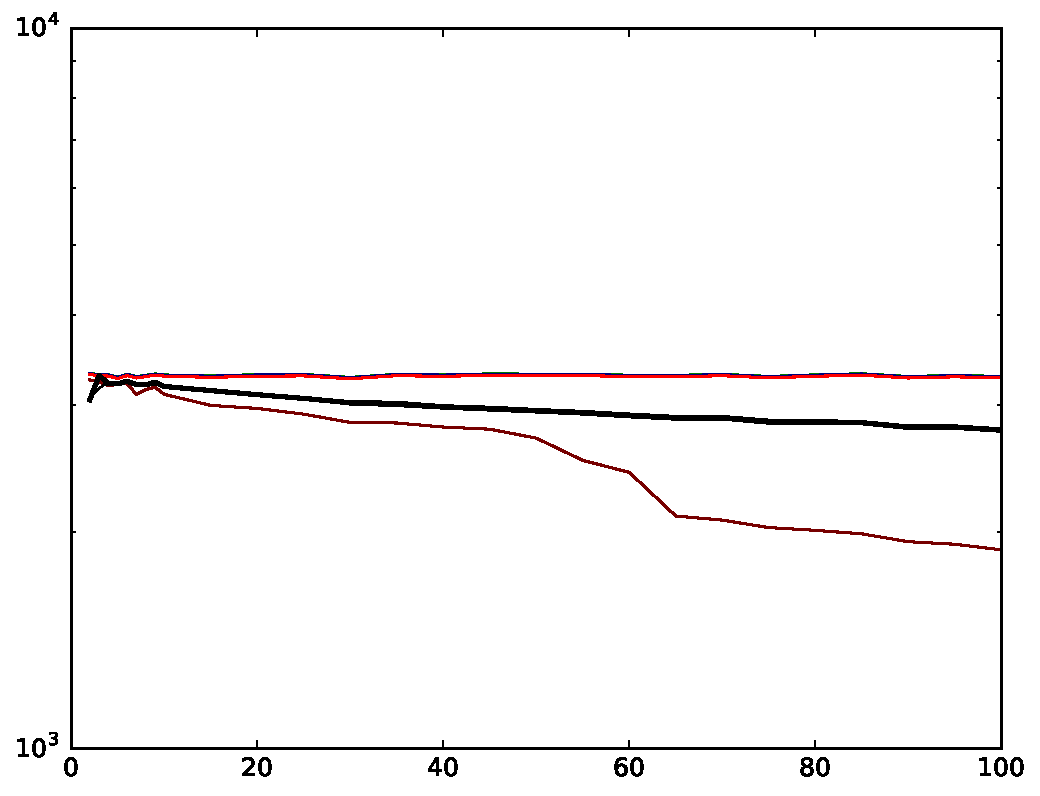
\includegraphics[width=0.3\textwidth]{img/logl2-auto-logl2-auto-uniform-log-1000-10000-star.pdf}
%\\
  %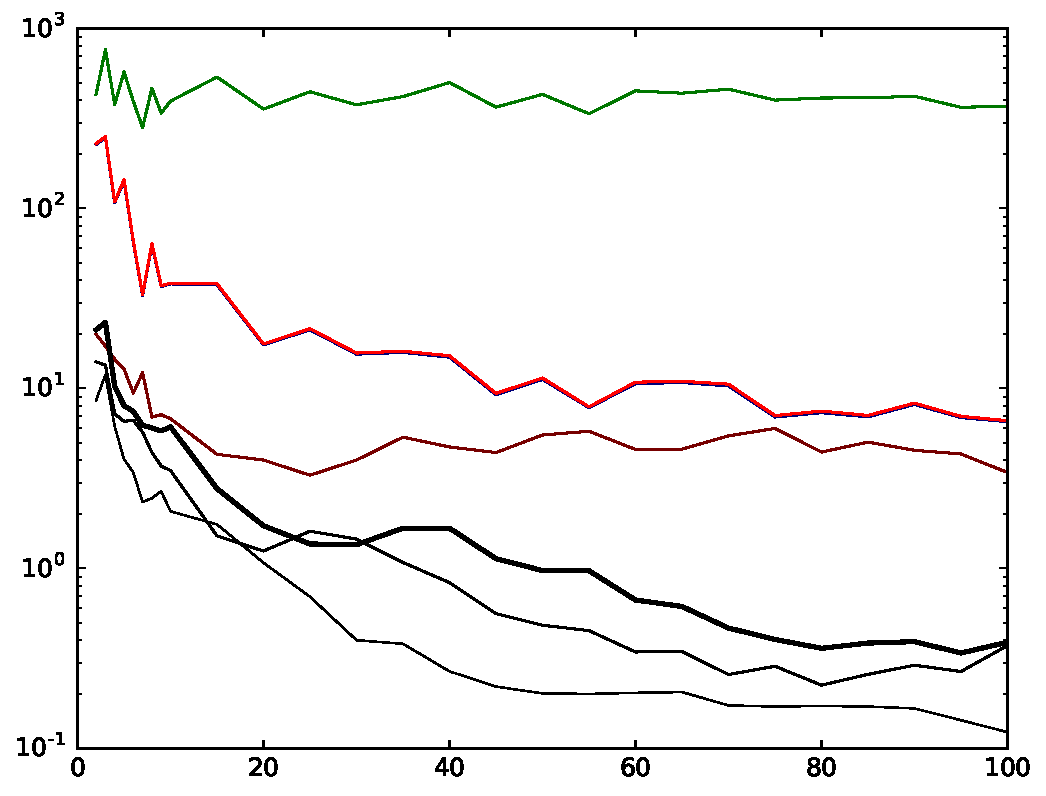
\includegraphics[width=0.3\textwidth]{img/logl1-auto-logl2-auto-laplace-log-1000-100-star.pdf}
%& 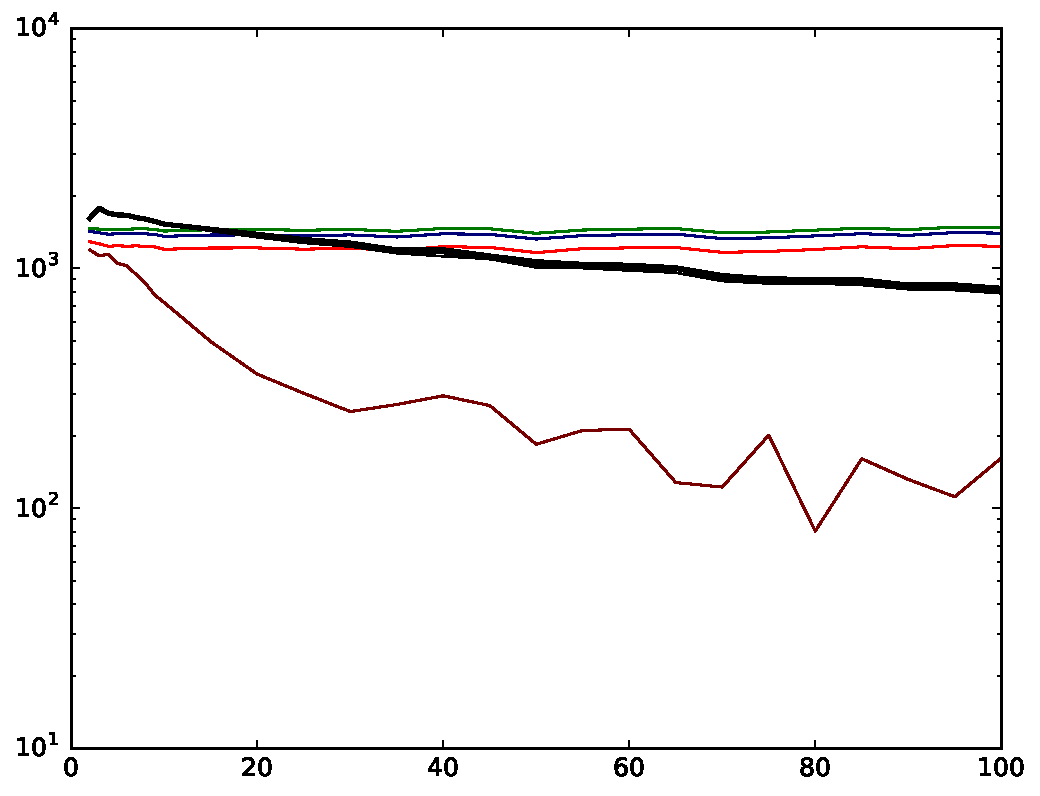
\includegraphics[width=0.3\textwidth]{img/logl1-auto-logl2-auto-laplace-log-1000-1000-star.pdf}
%& 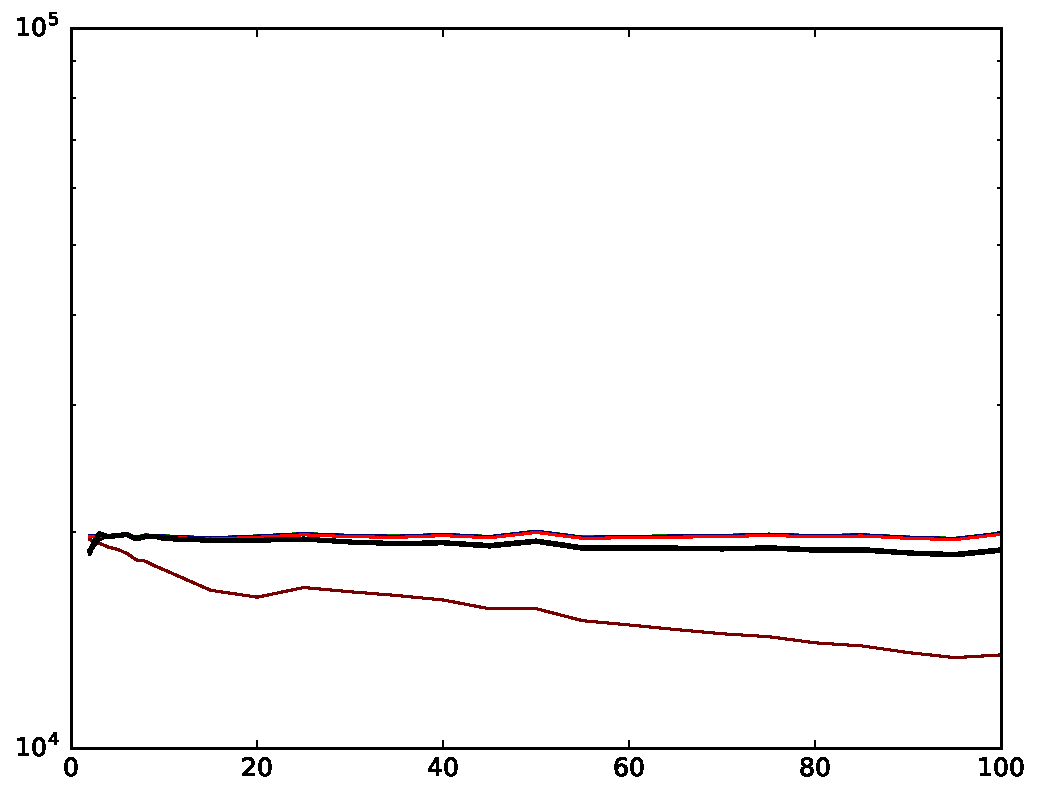
\includegraphics[width=0.3\textwidth]{img/logl1-auto-logl2-auto-laplace-log-1000-10000-star.pdf}
%\\
  %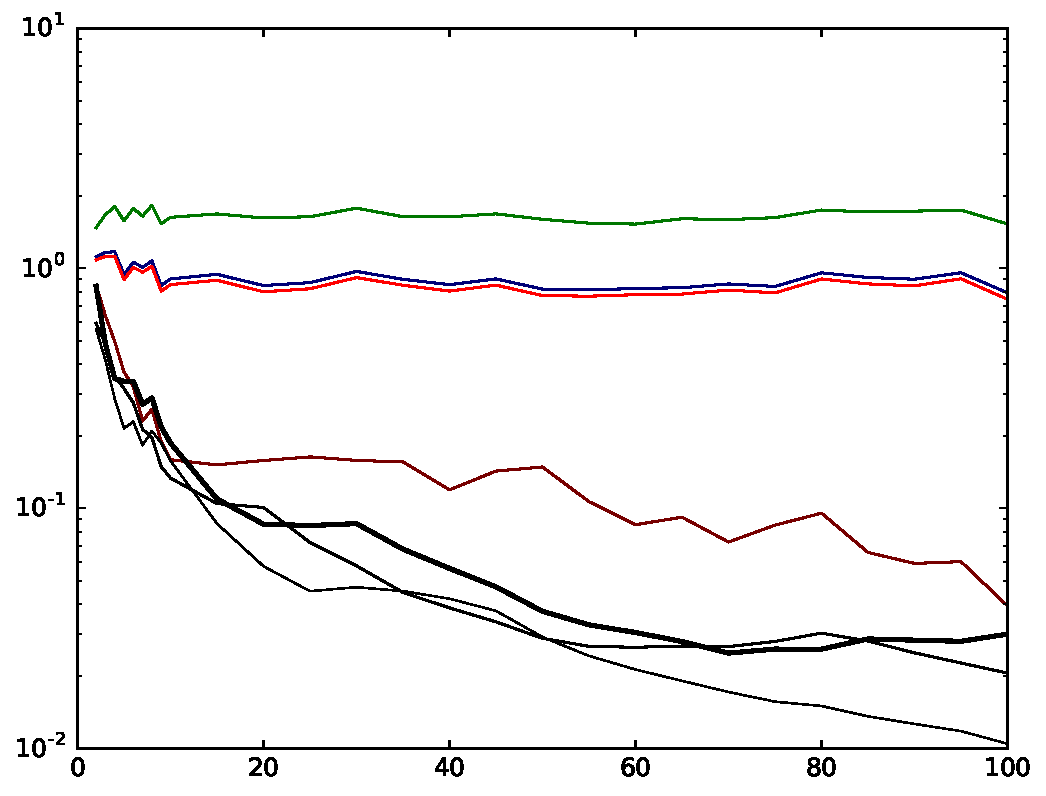
\includegraphics[width=0.3\textwidth]{img/logl1-auto-logl2-auto-spike-log-1000-100-star.pdf}
%& 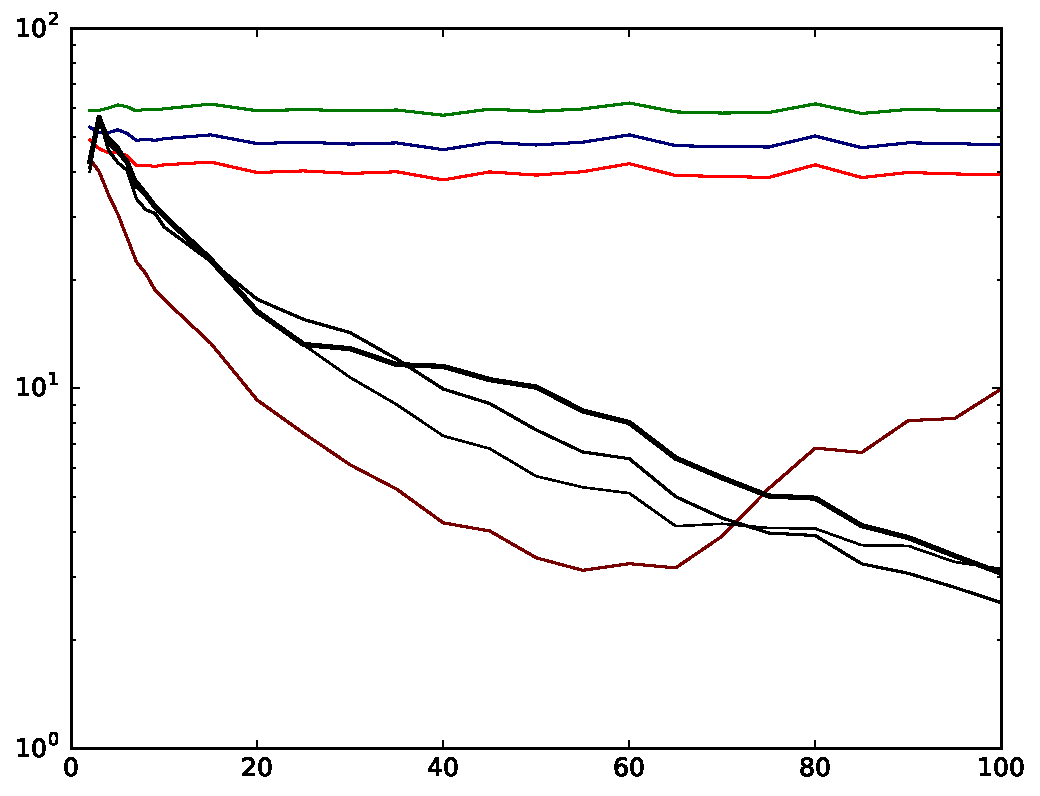
\includegraphics[width=0.3\textwidth]{img/logl1-auto-logl2-auto-spike-log-1000-1000-star.pdf}
%& 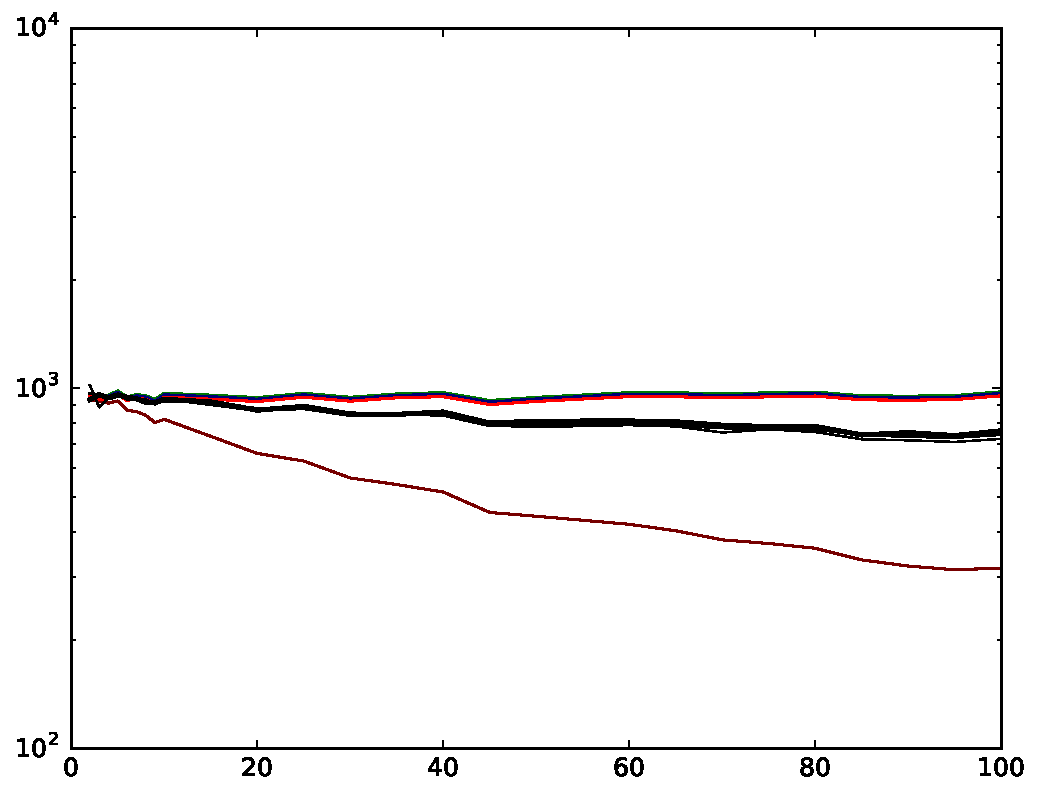
\includegraphics[width=0.3\textwidth]{img/logl1-auto-logl2-auto-spike-log-1000-10000-star.pdf}
%\end{tabular}
%\end{tikzpicture}
\plots{
\newcommand{\mklambdaplot}[4]{
\begin{tikzpicture}
    [ yscale=0.8
    ]
\tiny
#3
\begin{axis}
    [ width=0.35\textwidth
    %, xmode=log
    , ymode=log
    , xmin=1
    , xmax=100
#2
    ]
\addplot[black,no marks] table [x index=0,y index=5] {#1};
\addplot[brown,no marks] table [x index=0,y index=7] {#1};
\addplot[blue,no marks] table [x index=0,y index=9] {#1};
\addplot[red,thick,no marks] table [x index=0,y index=#4] {#1};
\addplot[darkgreen,very thick,no marks] table [x index=0,y index=55] {#1};
\addplot[dotted,darkgreen,very thick,no marks] table [x index=0,y index=56] {#1};
\addplot[darkgreen,very thin,no marks] table [x index=0,y index=56] {#1};
%\addplot[thick,red,no marks] table [x=n,y=bootll] {dat/kdd-scaling.dat};
%\addplot[very thick,darkgreen,no marks] table [x=n,y=owall] {dat/kdd-scaling.dat};
\end{axis}
\end{tikzpicture}
}
\begin{tabular}{cccc}
& $d=100$
& $d=1000$
& $d=10000$
\\
{\small\rotatebox{90}{\hspace{0.05cm}squared error $\ltwo{\wstar-\w}^2$}}
&\hspace{-0.5cm}\mklambdaplot
    {dat/logl1-auto-logl2-auto-spike-log-1000-100-star.pdf.csv}
    {,ymin=10^-2,ymax=10^1}
    { \node at (3,3) {\tiny\textcolor{brown}{$\wmle_i$}};
      \draw[->,brown] (2.7,2.85) -- (2.6,2.7);
      \node at (3.5,2.5) {\tiny\textcolor{blue}{$\wave$}};
      \draw[->,blue] (3.4,2.45) -- (3.45,2.35);
      \node at (2.5,1.9) {\tiny\textcolor{red}{$\wboot$}};
      \draw[->,thick,red] (2.5,2.0) -- (2.6,2.2);
      \node at (3.3,1.4) {\tiny$\wmle$};
      \draw[->] (3.2,1.3) -- (3.3,1.15);
      \node at (0.8,0.5) {\tiny\textcolor{darkgreen}{$\wowafull$}};
      \draw[->,darkgreen,dotted,thick] (0.8,0.65) -- (0.9,0.8);
      \draw[->,darkgreen,very thin] (0.8,0.65) -- (0.9,0.8);
      \node at (2.7,0.8) {\tiny\textcolor{darkgreen}{$\wowa$}};
      \draw[->,darkgreen,thick] (2.6,0.7) -- (2.7,0.55);
    }
    {19}
&\hspace{-0.5cm}\mklambdaplot
    {dat/logl1-autoreg-logl2-auto-spike-log-1000-1000-star.pdf.csv}
    {,ymin=10^0,ymax=10^2}
    {}
    {15}
&\hspace{-0.5cm}\mklambdaplot
    {dat/logl1-auto-logl2-auto-spike-log-1000-10000-star.pdf.csv}
    {}
    {}
    {11}
\\
& \hspace{0.2cm} {\small number of machines ($m$)}
&
&
\end{tabular}
}
\vspace{-0.15in}
\caption{
    $\wowa$ scales well with the number of machines.
    Surprisingly, it outperforms the oracle estimator trained on all of the data $\wmle$ in some situations.
    This is likely due to the additional regularization introduced by the OWA algorithm,
    as seen in Figure \ref{fig:lambda}.
    }
\label{fig:synscale}
\end{figure*}

We generate the data according to the following sparse logistic regression model.
Each component of the true parameter vector $\wstar$ is sampled i.i.d. from a spike and slab distribution.
With probability 0.9, the component is 0;
with probability 0.1, the component is sampled from a standard normal distribution.
The data points are then sampled as
\begin{equation}
\begin{aligned}
\x_i &\sim \normal{0}{I}
,
~~~
y_i = \left(1+\exp(-\trans\x_i\wstar)\right)^{-1}
.
\end{aligned}
\end{equation}
In all experiments, we use the L1 regularizer to induce sparsity in our estimates of $\wstar$.
Our estimators will be biased because the model is misspecified.
%(L1 regularization corresponds to a Laplace prior on the parameter vector.)
The true model for L1 regularization has a Laplace prior on $\wstar$.
%Results are qualitatively similar when using a uniform, normal, and Laplace prior on $\wstar$.
%These results are not shown due to space limitations.

Our first experiment shows the sensitivity of the estimators to the strength of regularization $\lambda$.
In this experiment, $\lambda$ was allowed to vary from $10^{-4}$ to $10^4$.
For each value of $\lambda$, we randomly generated 50 datasets (with $n=1000$) and then calculated the corresponding estimators.
Our $\wowa$ estimator was trained with $\nowa=128$.
Figure \ref{fig:lambda} shows the average of the results for three choices of $m$ and $d$.
Our $\wowa$ estimator is significantly less sensitive to the choice of $\lambda$ than the other distributed estimators.
Surprisingly, $\wowa$ even outperforms the oracle $\wmle$ in some regimes.
This is likely due to additional regularization induced by the approximation in Equation \ref{eq:approxreg}.

Our second experiment shows how the parallel algorithms scale as the number of machines $m$ increases.
We fix $n=1000$ data points per machine,
so the size of the dataset $mn$ grows as we add more machines.
This simulates the typical ``big data'' regime where data is abundant,
but processing resources are scarce.
Each machine independently uses cross validation to select the $\lambda$ that best fits the data locally.
There are three advantages to this model selection procedure.
First, there is no additional communication because model selection is a completely local task.
Second, existing optimizers have built-in model selection routines which make the process easy to implement.
We used the default model selection procedure from Python's SciKit-Learn \citep{scikit-learn}.
Third, the data may be best fit using different regularization strengths for each machine.
The results are shown in Figure \ref{fig:synscale}.
%The performance of our method scales well with the number of machines,
%and in some cases even outperforms the oracle trained on all of the data.
The performance of $\wowa$ scales much better than $\wave$ and $\wboot$.
Because of the regularization induced by Equation \ref{eq:approxreg} observed in the previous experiment,
$\wowa$ even scales better than $\wmle$ in some regimes.
%Surprisingly, matches (or exceeds) the performance of the oracle $\wmle$ as the number of machines $m$ increases.

%The advantage of artificial data is that we know the true model parameters and can evaluate our estimators' performance using the mean squared error.
%We test against two GLMs: an ordinary least squares regression and a logistic regression.
%In both experiments, we pick a constant dimension $d$ and a constant number of data points per machine $n$, then vary the number of machines $m$.
%In total, there are $mn$ data points for each trial.
%Each trial is repeated 100 times, and the reported results are the average.
%
%To evaluate the performance of our parallelization procedure, we evaluate against 4 baseline estimators.
%The first (Naive) is the performance of just a single machine on $n$ data points without merging the results.
%The second (Oracle) is the performance using all $mn$ data points on a single machine.
%For large values of $n$ or $m$ this would of course be impractical to calculate.
%The third (Ave) is the average of all the parameter vectors from each machine.
%The fourth (BootstrapAve) is evaluated according to the following procedure.
%Each machine $i$ calculates a parameter estimate $\theta_i$ using all the $n$ data points it has available,
%and a second estimate $\theta_i'$ using only $rn$ data points (where $r$ is a constant between 0 and 1).
%The final estimator is given by:
%
%$$
%\frac{\theta_i - r\theta_i'}{1-r}
%$$
%
%The idea of this procedure is to estimate the bias of the model using the smaller sample, and return a bias corrected estimate of the final procedure.
%In practice, the value of the $r$ parameter greatly affects the estimator's performance, and this parameter must be set by cross-validation.
%In our experiments, we use each of the values in the set $\{0.5,0.4,0.3,0.2,0.1,0.05,0.02,0.01,0.05\}$ and report only the best possible $r$ value.
%Our method has no similar parameters to tune, and tends to perform better than BootstrapAve even when the latter uses the optimal $r$ parameter.
%
%\subsubsection{Data from an ordinary leasts squares model}
%The true model parameters $\theta$ were generated according to one of three priors:
%the uniform distribution over $[0,1]$,
%the standard normal distribution,
%and the standard laplace distribution.
%Our data set $X$ was then generated from a standard normal distribution,
%and the corresponding $Y$ values sampled from $X^T\theta + h(X,\theta) + \epsilon$,
%where $\epsilon$ is the standard normal distribution.
%We use three different values of $h$ to evaluate the effect of incorrect modeling assumptions on our estimators.
%The function $h(X,\theta)=0$ tests the case when our model assumptions are correct.
%In this case, the OLS estimator is unbiased.
%%The function $h(X,\theta)=

\subsection{Real World Advertising Data}

\vspace{-0.1in}
We now evaluate our estimator on real world data from the KDD 2012 Cup \citep{kddcup2012}.
The goal is to predict whether a user will click on an ad from the Tencent internet search engine.
This dataset was previously used to evaluate the performance of $\wboot$ \citep{zhang2012communication}.
This dataset is too large to fit on a single machine.
There are 235,582,879 distinct data points,
each of dimension 741,725.
The data points are sparse, so we use the L1 norm to encourage sparsity in our final solution.
The regularization strength was set using cross validation in the same manner as for the synthetic data.
For each test, we split the data into 80 percent training data and 20 percent test data.
The training data is further subdivided into 128 partitions,
one for each of the machines used.

Our first experiment tests the sensitivity of the $\nowa$ parameter on large datasets.
We fix $m=128$, and allow $\nowa$ to vary from $2^0$ to $2^{20}$,
which is approximately the size of the full dataset.
We repeated the experiment 50 times, each time using a different randomly selected set $\Zowa$ for the second optimization.
Figure \ref{fig:nowa} shows the results.
Our $\wowa$ estimator has lower loss than the $\wave$ using only 16 data points per machine (approximately $4\times10^{-8}$ percent of the full training set)
and $\wowa$ has converged to its final loss value with only 1024 data points per machine (approximately $2.7\times10^{-6}$ percent of the full training set).
This justifies our claim that only a small number of data points are needed for the second round of optimization,
and so the communication complexity of $\wowa$ is essentially the same as $\wave$.

\begin{figure}[h!]
\plots{
\begin{tabular}{cc}
\rotatebox{90}{\hspace{1cm}log-loss}
&
\hspace{-0.5cm}
\begin{tikzpicture}
\small
\node at (2.5,1.5) {\tiny\textcolor{darkgreen}{$\wowa$}};
\draw[->,darkgreen,thick] (2.1,1.5) -- (1.85,1.5);
\node at (1,0.2) {\tiny\textcolor{red}{$\wboot$}};
\draw[->,red,thick] (0.6,0.25) -- (0.5,0.45);
\node at (1,1.1) {\tiny\textcolor{blue}{$\wave$}};
\draw[->,blue] (0.9,1) -- (1.0,0.85);
\begin{axis}
    [ width=0.45\textwidth
    , height=1.5in
    , xmin=1
    , xmax=1048576
    , ymin = 0.137
    , ymax = 0.14
    , y tick label style={
        /pgf/number format/.cd,
            fixed,
            fixed zerofill,
            precision=3,
        /tikz/.cd
    },
    , xtick={1,32,1024,32768,1048576}
    , log basis x={2}
    , xmode=log
    ]
%\addplot[blue,no marks] coordinates {(1,0.1376699823) (1048576,0.1376699823)};
%\addplot[thick,red,no marks] coordinates {(1,0.137198363008) (1048576,0.137198363008)};
%\addplot[very thick,darkgreen,no marks] table [x=nowa,y=128ll] {dat/kdd-nowa.dat};
\addplot[blue,no marks] coordinates {(1,0.138045477888) (1048576,0.138045477888)};
\addplot[thick,red,no marks] coordinates {(1,0.137682508908) (1048576,0.137682508908)};
\addplot[very thick,darkgreen,no marks] table [x=nowa,y=16ll] {dat/kdd-nowa.dat};
\end{axis}
\end{tikzpicture}
\\
&
\hspace{-0.15cm} data points used in second optimization $(\nowa)$
\end{tabular}
}
\vspace{-0.15in}
\caption{
    Relatively few data points are needed in the second round of optimization for $\wowa$ to converge.
    %Shown is the case when $m=16$.
    %Other values of $m$ are similar.
    }
\label{fig:nowa}
\end{figure}

\begin{figure}[h!]
\plots{
\begin{tabular}{cc}
\rotatebox{90}{\hspace{1cm}log-loss}
&
\hspace{-0.25cm}
\begin{tikzpicture}
\node at (5.3,0.75) {\tiny\textcolor{blue}{$\wave$}};
\draw[->,blue] (5.1,0.6) -- (5,0.4);
\node at (3.5,0.85) {\tiny\textcolor{red}{$\wboot$}};
\draw[->,red,thick] (3.2,0.7) -- (3,0.35);
\node at (0.5,0.35) {\tiny\textcolor{darkgreen}{$\wowa$}};
\draw[->,darkgreen, very thick] (0.5,0.5) -- (0.7,0.9);
\small
\begin{axis}
    [ width=0.45\textwidth
    , height=1.5in
    , xmin=2
    , xmax=128
    , ymin = 0.137
    , ymax = 0.142
    , ytick={0.137,0.138,0.139,0.14,0.141,0.142}
    , y tick label style={
        /pgf/number format/.cd,
            fixed,
            fixed zerofill,
            precision=3,
        /tikz/.cd
    },
    %, xtick={2,4,128}
    , log basis x={2}
    , xmode=log
    ]
\addplot[blue,no marks] table [x=n,y=avell] {dat/kdd-scaling.dat};
\addplot[thick,red,no marks] table [x=n,y=bootll] {dat/kdd-scaling.dat};
\addplot[very thick,darkgreen,no marks] table [x=n,y=owall] {dat/kdd-scaling.dat};
\end{axis}
\end{tikzpicture}
\\
&
\hspace{0.5cm}number of machines ($m$)
\end{tabular}
}
\vspace{-0.15in}
\caption{
    Performance of the parallel estimators on advertising data as the number of machines $m$ increases.
    }
\label{fig:kdd-scaling}
\end{figure}

Our last experiment shows the performance as we scale the number of machines $m$.
The results are shown in Figure \ref{fig:kdd-scaling}.
Here, our $\wowa$ performs especially well in the low $m$ setting.
For large $m$, $\wowa$ continues to slightly outperform $\wboot$ without the need for an expensive model selection procedure to determine the $r$ parameter.

\section{CONCLUSION}

\vspace{-0.1in}
We introduced a new distributed estimation algorithm called OWA.
OWA has the speed advantages of non-interactive distributed estimators,
but has better accuracy due to a (cheap) second round of optimization.
% cshelton: hmmm... how about not requiring any *global* cross validation
% (that is xv that depends on the entire dataset)?
Unlike other algorithms, OWA does not require expensive hyperparameter tuning.
Furthermore, our analysis is more general than the analysis of similar algorithms.
As part of our analysis, we also provided a more general analysis of the averaging estimator.

%We do not require the likelihood to be convex.
%OWA uses two rounds of communication,
%so it is not subject to existing regret bounds for non-interactive learners.
%The second round of communication requires little communication, however,
%so we maintain the advantages of non-interactive distributed learning.

%%%%%%%%%%%%%%%%%%%%%%%%%%%%%%%%%%%%%%%%%%%%%%%%%%%%%%%%%%%%%%%%%%%%%%%%%%%%%%%%

\clearpage
\bibliographystyle{plainnat}
\bibliography{paper}

%%%%%%%%%%%%%%%%%%%%%%%%%%%%%%%%%%%%%%%%%%%%%%%%%%%%%%%%%%%%%%%%%%%%%%%%%%%%%%%%

\clearpage

\section*{Appendix: Proof of Theorem 1}
We have by the triangle inequality that
\begin{equation}
\ltwo{\wstar-\wave} \le \ltwo{\wstar-\E\wave} + \ltwo{\E\wave-\wave}
.
\label{eq:biasvar}
\end{equation}
The left term above captures the estimator's bias and the right term the variance.
First we consider the bias.
By the linearity of expectation, we have that
\begin{align}
\E\wave
&=
\E\frac{1}{m}\sum_{i=1}^m\wmle_i
%\\&=
=
\frac{1}{m}\sum_{i=1}^m\E\wmle_i
=
\E\wmle_i
,
\label{eq:expwave}
\end{align}
and so the bias term
$\ltwo{\wstar-\E\wave}
=
\ltwo{\wstar-\E\wmle_i}
$.
%In words, the bias of the combined averaging estimator is the same as the bias of the estimator on an individual machine.

Now we consider the variance.
We have that
\begin{align}
&\ltwobig{\wave-\E\wave}
\\&=
%\frac{1}{m}\sum_{i=1}^m\wmle_i-\E\wave
%\\&=
\ltwobig{\frac{1}{m}\sum_{i=1}^m\wmle_i-\E\wave}
\label{eq:var1}
\\&=
\frac{1}{m}\ltwobig{\sum_{i=1}^m\left(\wmle_i-\E\wmle_i\right)}
%\\&=
%\frac{1}{m}\ltwobig{\sum_{i=1}^m\I^{-1/2}_\wstar\I^{1/2}_\wstar\left(\wmle_i-\E\wmle_i\right)}
\\&=
\frac{1}{m\sqrt{n}}\ltwobig{\I^{-1/2}_\wstar\sum_{i=1}^m\sqrt{n}\I^{1/2}_\wstar\left(\wmle_i-\E\wmle_i\right)}
\\&=
\frac{1}{m\sqrt{n}}\ltwobig{\I^{-1/2}_\wstar\sum_{i=1}^m\Delta_{\wmle_i}}
\label{eq:var1}
.
\end{align}
%Equation \ref{eq:var1} follows by multiplying inside the norm by $1=\sqrt{n}\I_{\wstar}^{1/2}\I_{\wstar}^{-1/2}/\sqrt{n}$ and applying the definition of $\Delta_{\wmle_i}$.
Notice that each of the $\Delta_{\wmle_i}$ are i.i.d.\ sub-Gaussian random vectors.
Sub-Gaussian random vectors inherit the following basic property from centered Gaussian random vectors:
The sum of $m$ i.i.d.\ sub-Gaussians has the same distribution as $\sqrt{m}$ times the sub-Gaussian.
% cshelton: what is Delta_1?  Is it defined just as the rv that causes
% the sum to be distributed portionally to it?  Perhaps we can clarify?
That is, $\sum_{i=1}^m \Delta_{\wmle_i} \sim \sqrt{m}\Delta_{\wmle_1}$.
Substituting into Equation \ref{eq:var1} gives
\begin{equation}
\ltwobig{\wave-\E\wave}
\sim
\frac{1}{\sqrt{mn}}\ltwobig{\I^{1/2}_\wstar\Delta_{\wmle_1}}
.
\label{eq:var2}
\end{equation}

%Centering the distribution and applying Equation \ref{eq:expwave} gives
%\begin{equation}
%\E\wave-\wave
%\sim
%\normal{\zero}{\frac{1}{nm}I^{-1}}
%\end{equation}
%In the last step we used the fact that adding a sub-Gaussian random variable to itself $m$ times is equivalent lto multiplying the Gaussian by $\sqrt{m}$.
%So bounding the variance reduces to bounding the norm of a Gaussian.

Our last step is to bound the norm on the right hand side of Equation \ref{eq:var2}.
Theorem 2.1 from \cite{hsu2012tail} gives a bound on the norm of a positive semidefinite matrix times a sub-Gaussian random variable.
Applying the theorem gives that %with probability at least $1-\exp(-t)$,
\begin{equation}
\prob{
    \ltwobig{\I^{-1/2}_\wstar\Delta_1} < \sqrt{v_t}
}
\ge 1-\exp(-t)
,
\end{equation}
where $v_t$ is defined as in Equation \ref{eq:vt}.
And so the variance of $\wave$ satisfies
\begin{equation}
\prob{
\ltwobig{\wave-\E\wave}
<
\sqrt\frac{v_t}{{mn}}
}
\ge 1-\exp(-t)
.
\label{eq:ct1}
\end{equation}
%and so
%\begin{equation}
%\ltwo{\E\wave-\wave} \le \sqrt\frac{v_t}{nm}
%\label{eq:ct1}
%\end{equation}
%where
%\begin{equation}
%\begin{aligned}
%v_t'
   %= \tr\left({\frac{1}{mn}\I^{-1}_{\wtave}}\right)
%+ 2&\sqrt{\tr \left({\frac{1}{mn}\I^{-1}_{\wtave}}\right)^2t}&
%\\+ 2\ltwo{\frac{1}{nm}\I^{-1}_{\wtave}}t&
%\end{aligned}
%\end{equation}
%Then by the linearity of trace and scalability of norms,
%\begin{equation}
%v_t' =
%\frac{1}{mn}\left(
%\tr\I^{-1}_{\wtave}
%+ 2\sqrt{\tr \I^{-2}_{\wtave}t}
%+ 2\ltwo{\I^{-1}_{\wtave}}t
%\right)
%\label{eq:ct2}
%\end{equation}
Substituting Equations \ref{eq:expwave} and \ref{eq:ct1} into Equation \ref{eq:biasvar} gives the stated result.

\section*{Appendix A: Proof of Lemma 1}

Define the space $\Gamma=\vecspan\{\wmle_i-\E\wave\}_{i=1}^m$.
Our proof strategy is to bound the distance $\ltwo{\wstar-\proj\Gamma\wstar}$ and then show that $\Gamma\approx\W$.
Specifically, we have
\begin{align}
~~~~&\!\!\!\!\!\!\!\!\!\!\!\!\!%\!\!\!\!\!\!\!
\ltwo{\wstar-\proj\W\wstar}
\nonumber
\\
&=
\ltwo{(\wstar-\wave) - (\proj\W\wstar - \wave)}
%\nonumber
\\
&=
\ltwo{(\wstar-\wave) - \proj\W(\wstar - \wave)}
\label{eq:waveinW}
\\
&\le
\ltwo{(\wstar-\wave) - \proj\W\proj\Gamma(\wstar - \wave)}
\label{eq:addprojGamma}
\\
&\le
\ltwo{(\wstar-\wave) - \proj\Gamma(\wstar-\wave)}
\nonumber
\\
&~~~+
\ltwo{\proj\Gamma(\wstar-\wave) - \proj\W\proj\Gamma(\wstar-\wave)}
%\ltwo{\proj\Gamma(\wstar-\wave) - \proj\W(\wstar-\wave)}
%\label{eq:gammatriangle}
%\\
%&=
%\ltwo{(I-\proj\Gamma)(\wstar - \wave)}
%\nonumber
%\\
%&~~~+
%\ltwo{(\proj\Gamma-\proj\W)(\wstar - \wave)}
.
\label{eq:i-projW}
\end{align}
Equation \ref{eq:waveinW} follows because $\wave\in\W$;
Equation \ref{eq:addprojGamma} by the definition of $\proj\W$;
and Equation \ref{eq:i-projW} by the triangle inequality.
%Recall that we defined $\matW$ to be the $d\times m$ matrix with $i$th column equal $\wmle_i$.
%The column space of $\matW$ is $\W$.
We now bound each of the terms in Equation \ref{eq:i-projW} separately,
beginning with the leftmost.

%We can write
%\begin{equation}
%\proj\Gamma = \Delta_{\wmle_i}
%\end{equation}
Define the matrix $G$ with $i$th column equal to the vector $(\wmle_i-\E\wmle_i)$.
The column space of $G$ is $\Gamma$,
and we have that
%$\proj\Gamma=G\pinv G$.
\begin{align}
\proj\Gamma
&=
G\pinv G
\\
&= \I_\wstar^{-1/2}\bigg(\sqrt{n}\I_\wstar^{1/2}G\bigg)
             \pinv{\bigg(\sqrt{n}\I_\wstar^{1/2}G\bigg)}
   \I_\wstar^{1/2}
,
\label{eq:ggpinv}
\end{align}
where the superscript $\pinv{}$ denotes the Moore-Penrose pseudoinverse.
The $i$th column of matrix $\sqrt{n}\I^{1/2}_{\wstar}G$ is equal to $\Delta_{\wmle_i}$ by definition.
%
%So the projection $\proj\W = \matW\pinv\matW$, where the superscript $\pinv{}$ is the Moore-Penrose pseudoinverse.
%Define the matrix $\matV=\sqrt{n}I^{1/2}\matW$.
%Then the columns of $\matV$ are sub-Gaussian by the SGT condition,
%and we can write
%\begin{equation}
%\proj\W
%= \I^{-1/2} \matV \pinv\matV \I^{1/2}
%.
%\label{eq:vvp}
%\end{equation}
Let $U\Sigma \trans V$ be the singular value decomposition of $\sqrt{n}\I^{1/2}_{\wstar}G$,
where $U$ and $V$ are orthogonal matrices and $\Sigma$ is the diagonal matrix of singular values.
Substituting into Equation \ref{eq:ggpinv} gives
\begin{align}
\proj\Gamma
&= \I^{-1/2} (U\Sigma \trans V)\pinv{(U \Sigma \trans V)} \I^{1/2}
\\
&= \I^{-1/2} (U\Sigma \trans V)(V \pinv\Sigma \trans U) \I^{1/2}
\\
&= \I^{-1/2} U\Sigma \pinv\Sigma \trans U \I^{1/2}
.
\label{eq:vvp2}
\end{align}
%Substituting Equation \ref{eq:vvp2} into \ref{eq:i-projW} gives
This implies that
\begin{align}
%~~~~~&\!\!\!\!\!\!\!\!\!\!\!\ltwo{\wstar-\proj\Gamma\wstar}
~~~~~&\!\!\!\!\!\!\!\!\!\!\!\ltwo{(I-\proj\Gamma)(\wstar-\wave)}
\nonumber
\\
&=
\ltwo{(I-\I^{-1/2} U\Sigma \pinv\Sigma \trans U \I^{1/2})(\wstar - \wave)}
\\
&=
\ltwo{\I^{-1/2} U(I-\Sigma \pinv\Sigma )\trans U \I^{1/2}(\wstar - \wave)}
\\
&=
\sqrt{\smin}\ltwo{U(I-\Sigma \pinv\Sigma )\trans U \I^{1/2}(\wstar - \wave)}
\label{eq:fromdefsmin}
\\
&=
\sqrt{\smin}\ltwo{(I-\Sigma \pinv\Sigma )\trans U \I^{1/2}(\wstar - \wave)}
\label{eq:fromrotinvl2}
.
\end{align}
Equation \ref{eq:fromdefsmin} follows from the definition of $\smin$ as the smallest eigenvector of $\I$,
and Equation \ref{eq:fromrotinvl2} follows from the rotational invariance of the L2 norm.
The matrix $(I-\Sigma\pinv\Sigma)$ contains 1s in the first $d-m$ diagonal entries, and zeros everywhere else.
By the rotational invariance of the sub-Gaussian distribution (Lemma 5.9 of Vershynin, 2011),
$U$ and $V$ are distributed uniformly over the orthogonal group of matrices.
%Because $U$ is distributed uniformly over the orthogonal group,
Therefore the operator $(I-\Sigma\pinv\Sigma)\trans U$ projects a vector onto a subspace of dimension $d-m$ chosen uniformly at random.
Lemma 2.2 from \cite{dasgupta2003elementary} provides a bound for this situation.
The lemma states that for any vector $\x$, for all $t>0$, with probability at least $1-\exp((d-m)(-t+\ln (t+1)))$,
\begin{align}
\ltwo{(I-\Sigma\pinv\Sigma)\trans U \x} \le (t+1) \sqrt{1-\frac{m}{d}}
.
\label{eq:dasgupta}
\end{align}
%Substituting gives
%Applying Equation \ref{eq:dasgupta} to \ref{eq:blurby} gives
Setting $\x=\I^{1/2}(\wstar-\wave)$ gives
\begin{align}
~~~~~&\!\!\!\!\!\!\!\!\!\!\!\ltwo{(I-\proj\Gamma)(\wstar-\wave)}
\nonumber
\\
&\le
(t+1)\sqrt{\smin\left(1-\frac{m}{d}\right)}\ltwo{\I^{1/2}(\wstar - \wave)}
\\
&\le
(t+1)\sqrt{\frac{\smin}{\smax}\left(1-\frac{m}{d}\right)}\ltwo{\wstar - \wave}
,
\end{align}
which bounds the leftmost term of Equation \ref{eq:i-projW}.

%Now we bound the rightmost term.
%We have that
%%\begin{align}
%%\proj\Gamma(\wstar-\wave)
%%&=
%%\sum_{i=1}^m a_i (\wmle_i - \E\wmle_i)
%%\\
%%\proj\Gamma(\wstar-\wave)+\sum_{i=1}^m a_i(\E\wmle_i - \wave)
%%&=
%%\sum_{i=1}^m a_i (\wmle_i - \wave)
%%\end{align}
%\begin{align}
%~~~~~~~~~~~~~~~~~&\!\!\!\!\!\!\!\!\!\!\!\!\!\!\!\!\!\!\!\!\!\!\!\!\!\!\!\!\!\!\!\!\!\!\!\!\!\!\ltwo{\proj\Gamma(\wstar-\wave)-\proj\W\proj\Gamma(\wstar-\wave)}
%\nonumber
%\\
%&\le
%\ltwo{\E\wmle_i-\wave}\ltwo{\proj\Gamma(\wstar-\wave)}
%\\
%&\le
%\ltwo{\E\wmle_i-\wave}\ltwo{\wstar-\wave}
%\\
%&\le
%\frac{v_t}{\sqrt{mn}}\ltwo{\wstar-\wave}
%\end{align}
%Substituting Equations 47 and 50 into 35 gives the stated result.

%%%%%%%%%%%%%%%%%%%%%%%%%%%%%%%%%%%%%%%%

\section*{Appendix B: Proof of Lemma 2}
By the triangle inequality, we have that
\begin{align}
\ltwo{\wstar-\wowa}
\le
\ltwo{\wowastar-\wowa}
+
\ltwo{\wstar-\wowastar}
.
\label{eq:wstarwowa}
\end{align}
We bound the right hand term as follows.
By the definition of $\qhi$ and $\qlo$, we have
\begin{align}
\qlo \left( \ltwo {\wstar-\wowastar} \right)
&\le F(\wstar) - F(\wowastar)
\\
&\le F(\wstar) - F(\proj\W\wstar)
\\
&\le \qhi \left( \ltwo {\wstar - \proj\W\wstar} \right)
.
\end{align}
%and so
%\begin{equation}
%\ltwo {\wstar-\wowastar}
%\le
%\qlo^{-1} \left(
    %\qhi \left( \ltwo {\wstar - \proj\W\wstar} \right)
%\right)
%.
%\end{equation}
%Applying Lemma \ref{lem:proj} gives the stated result.
Applying $\qlo^{-1}$ to both sides and substituting into Equation \ref{eq:wstarwowa} gives the stated result.

\end{document}
